\documentclass[10pt,a4paper]{article}
\usepackage[utf8]{inputenc}
\usepackage[T1]{fontenc}
\usepackage[margin=0.82in,top=0.7in,bottom=0.7in]{geometry}
\usepackage{amsmath}
\usepackage{amssymb}
\usepackage{graphicx}
\usepackage{booktabs}
\usepackage{xcolor}
\usepackage{hyperref}
\usepackage{xurl}
\usepackage{float}
\usepackage{array}
\usepackage{caption}
\usepackage{subcaption}
\usepackage{enumitem}
\usepackage{titlesec}
\usepackage{fancyhdr}
\usepackage{lastpage}

\usepackage{polyglossia}
\setdefaultlanguage{english}
\setotherlanguages{hindi,telugu}
\usepackage{fontspec}
\newfontfamily\teluguFont[Script=Telugu]{Noto Sans Telugu}
\newfontfamily\devanagariFont[Script=Devanagari]{Noto Sans Devanagari}

\setlength{\parindent}{0pt}
\setlength{\parskip}{3pt}
\titlespacing*{\section}{0pt}{8pt}{4pt}
\titlespacing*{\subsection}{0pt}{6pt}{3pt}
\titlespacing*{\subsubsection}{0pt}{4pt}{2pt}
\renewcommand{\arraystretch}{1.05}

\pagestyle{fancy}
\fancyhf{}
\rhead{\small LMA Individual Project --- Final Report}
\lhead{\small Phase 1--3 Consolidated}
\cfoot{\small\thepage/\pageref{LastPage}}
\renewcommand{\headrulewidth}{0.3pt}

\title{\vspace{-1.3cm}\textbf{\large Language Models and Agents Individual Project}\\[2pt]
\textbf{\Large Building and Analyzing Monolingual Transformer LMs in Two Indian Languages}\\[2pt]
\normalsize Consolidated Final Report (Phases 1--3 + Bonus Ablation)}
\author{\small Kspsvln Siddardha Kumar Kavuri \quad Roll No. 2025201061 \quad \texttt{kspsvlnsiddardha.k@students.iiit.ac.in}}
\date{\small \today}

\begin{document}
\maketitle
\thispagestyle{fancy}
\vspace{-0.9cm}


\section{Overview}
\vspace{-2pt}
Phase 1 (Sec.~\ref{sec:phase1}) builds independent corpora and tokenizers for Telugu
and Bhojpuri. Phase 2 (Sec.~\ref{sec:phase2}) implements the Transformer from scratch, pretrains
four models (two languages $\times$ two parameter scales), and evaluates them via
(perplexity/BPB) and generation quality, diversity, and attention analysis. Phase 3
(Sec.~\ref{sec:phase3}) finetunes each pretrained model on a synthetic reasoning task and
re-analyzes attention pre-/post-finetune. Also Sec.~\ref{sec:bonus} documents the optional
no-positional-embeddings ablation, and at last Sec.~\ref{sec:ablation-summary} indexes all four ablation
studies run across the project (tokenizer/vocab, parameter count at pretraining, parameter count
at finetuning, and this bonus one) in one place. Sec.~\ref{sec:discussion} answers the four
required comparison questions.

\section{Phase 1: Data Collection and Tokenizer Construction}
\label{sec:phase1}
\vspace{-2pt}
\textbf{Collection.} Telugu's Phase 1 collection included an existing 21.46M-line
manually-assembled corpus (\texttt{telugu.txt}, comfortably satisfying the $\geq$20\% manual-collection
requirement on its own) plus Wikipedia/news web-scraping (29,206 cleaned texts, 89.7\% pass
rate) and OCR augmentation (3.77M lines from archive.org), 25.35M lines in total. Also included Indica corp V2 telugu data\textbf{This
large manual corpus was collected in Phase 1 but was not carried into later phases}: the actual
train/val/test files used for Phase 2 pretraining (\texttt{telugu/data/\{train,val,test\}/telugu.txt})
are a separately-prepared, much smaller 3.89M-line corpus, so the 25.35M-line/4.42B-token
collection total below does not describe what the models were actually trained on -- see
Table~\ref{tab:pretrain-results} and Sec.~\ref{sec:phase2} for the real, used token counts.
Bhojpuri, the designated lower-resource language, combines a HuggingFace corpus
(\texttt{Satyam810/BhojpuriCorpus}, $\sim$261K lines), OCR extraction from Hindi archive.org
texts (511,599 lines), English$\to$Bhojpuri and Hindi$\to$Bhojpuri machine translation
(NLLB-200; 711,138 + 15,852 lines), and targeted web scraping (3,234 cleaned texts, 97.2\% pass
rate), for 1.83M total lines -- and unlike Telugu, Bhojpuri's entire collected corpus \emph{is}
the one actually used for pretraining (its train/val/test files match the collected total
exactly).

\textbf{Cleaning.} A 7-stage pipeline (Unicode NFD normalization, citation/control-character
removal, character whitelisting, script validation, length/word-count/density filters, MD5
deduplication, MinHash Deduplication) is applied identically to both languages, followed by a deterministic 80/10/10
train/val/test split (seed 42, whole-line preservation, no cross-split leakage).

\begin{table}[H]\centering\footnotesize
\begin{tabular}{lrrrr}
\toprule
Language & Train/val/test lines (used)$^\dagger$ & Total lines & Est.\ train/val/test tokens$^\ddagger$ & Total tokens \\
\midrule
Telugu (H)   & 3.11M / 389K / 389K & 3.89M & 407.7M / 50.9M / 50.7M & 509.3M \\
Bhojpuri (L) & 1.46M / 182K / 183K & 1.83M & 233.4M / 29.1M / 29.2M & 291.7M \\
\bottomrule
\end{tabular}
\caption{Corpus actually used for Phase 2 pretraining (Sec.~\ref{sec:phase2}), verified
directly from the real \texttt{\{telugu,bhojpuri\}/data/\{train,val,test\}/\{telugu,bhoj\}.txt}
files on disk. $^\dagger$Telugu's \texttt{config.json} separately lists a stale,
never-materialized 20.28M/2.53M/2.53M split describing the full 25.35M-line \emph{collected}
corpus above, not this actually used one not shown here since it was never trained on.
$^\ddagger$Token counts use Phase 1's own corpus-level estimator (total bytes / 4, matching the
\texttt{len(text)//4} convention in \texttt{data\_cleaner.py}/\texttt{enhanced\_scraper.py}) --
tokenizer-independent by design, so directly comparable across the two languages' different
WordPiece vocabularies; this is not the same as either model's own real subword-token count at
training time (Sec.~\ref{sec:phase2}), which varies by vocabulary size. Full
Phase 1 collection statistics (all sources, cleaning pass rates): \texttt{report/phase-1/phase1\_report.pdf}.}
\end{table}
\vspace{-8pt}

\subsection*{Ablation Study 1: Tokenizer Family and Vocabulary Size}
Three tokenizer families (byte-level BPE, Unicode-level BPE, WordPiece) were trained from scratch
and compared per language at exploratory vocabulary sizes, measuring fertility (avg.\ characters
per token) and UNK rate on held-out text.

\begin{table}[H]\centering\footnotesize
\begin{tabular}{llrrr}
\toprule
Language & Tokenizer family (vocab size) & Unique tokens used & Chars/token & UNK rate \\
\midrule
Telugu   & Byte-level BPE (50K)   & 1,978  & 1.33 & 0.0000\% \\
Telugu   & Unicode-level BPE (50K)& 11,398 & 5.93 & 0.0000\% \\
Telugu   & WordPiece (50K)        & 9,539  & 5.84 & 0.0000\% \\
Bhojpuri & Byte-level BPE (8K)    & 7,761  & 1.54 & 0.0000\% \\
Bhojpuri & Unicode-level BPE (32K)& 31,258 & 4.35 & 0.0000\% \\
Bhojpuri & WordPiece (32K)        & 25,000 & 3.95 & 0.0002\% \\
\bottomrule
\end{tabular}
\caption{Tokenizer-family/vocabulary ablation (Phase 1, exploratory sizes; full tables:
\texttt{report/phase-1/phase1\_report.pdf} Sec.\ 6).}
\label{tab:tok-ablation}
\end{table}
\vspace{-8pt}

Byte-level BPE is the most compact (fewest chars/token, i.e.\ most tokens per character of text)
but destroys word-boundary information also token generation is more for same sentence. Unicode-level BPE and WordPiece both preserve
linguistically meaningful subwords at comparable fertility ($\sim$4--6 chars/token). WordPiece was
selected for both languages for its explicit subword-continuation marking, which
Sec.~\ref{sec:phase2}'s exact-match scoring later depends on. \textbf{A second, independent
vocabulary-size ablation} happens implicitly across the four pretrained models themselves
(Sec.~\ref{sec:phase2}): WordPiece tokenizers were retrained from scratch at each model's own
target vocabulary rather than reusing one shared tokenizer 10,000 (Telugu/Bhojpuri
low-parameter pair, identical size, separate vocabularies), 20,000 (Telugu high-parameter), and
16,000 (Bhojpuri high-parameter) -- so vocabulary size also varies as one axis of the
parameter count ablation below.

\section{Phase 2: Model Implementation, Pretraining, and Evaluation}
\label{sec:phase2}
\vspace{-2pt}
\subsection{Architecture (implemented from scratch)}
A decoder-only, GPT-style Transformer: token embeddings + learned absolute positional
embeddings (chosen over sinusoidal/RoPE for simplicity and to let each model adapt position
representations to its own language; this fixes the maximum sequence length to the embedding
table size, 128 or 256 tokens depending on variant), summed and passed through $N$ pre-norm
blocks, each with manual multi-head causal self-attention and a GELU feedforward network, ending
in a final LayerNorm and a tied ($W_{\text{LM-head}} = W_{\text{token-embed}}^\top$) output
projection.
\vspace{-2pt}
\[
\text{Attention}(Q,K,V) = \text{softmax}\!\left(\frac{QK^\top}{\sqrt{d_k}} + M\right)V,
\qquad M_{ij} = \begin{cases}0 & j \le i\\ -\infty & j > i\end{cases}
\]
empirically: perturbing token $t{+}1$ leaves logits at position $t$ unchanged. Pre-norm
($x' = x + \text{Attn}(\text{LN}(x))$) was chosen over post-norm for training stability in a
deep stack. Cross-entropy on next-token logits is the sole training objective.

\subsection{Ablation Study 2: Parameter Count (Model Configurations and Pretraining Setup)}
Four independently trained checkpoints exist: an architecture-matched \emph{low-parameter} pair
(built first, for a clean resource-tier comparison ans phase-2 submission was based on this) and a separately-sized, larger
\emph{high-parameter} pair per language, trained with everything else (data pipeline, optimizer,
schedule shape) held fixed so parameter count (and its associated vocabulary size, dropped in as part of scaling up each architecture) is the isolated variable.

\begin{table}[H]\centering\footnotesize
\begin{tabular}{lrrrr}
\toprule
 & Telugu low & Telugu high & Bhojpuri low & Bhojpuri high \\
\midrule
Vocab (WordPiece) & 10,000 & 20,000 & 10,000 & 16,000 \\
$d_{\text{model}}$ / layers / heads & 256 / 6 / 8 & 384 / 10 / 8 & 256 / 6 / 8 & 320 / 8 / 8 \\
$d_{\text{ff}}$ / max seq len & 1024 / 128 & 1536 / 256 & 1024 / 128 & 1280 / 256 \\
Tied embeddings & yes & yes & yes & yes \\
\textbf{Parameters (verified)} & \textbf{7.34M} & \textbf{25.54M} & \textbf{7.34M} & \textbf{15.08M} \\
\bottomrule
\end{tabular}
\caption{Model configurations, all four pretrained variants.}
\end{table}
\vspace{-8pt}

All 4 Models were trained on same hyperparameter that is not change in these models: AdamW, cosine-annealing-with-linear-warmup schedule, batch size 32,
gradient clipping at 1.0, mixed precision, checkpoints containing weights + optimizer/scheduler
state + step/epoch + config (mandatory checkpoint-resume, exercised in practice across multiple
interrupted Kaggle sessions). Low-parameter pair: LR $1\times10^{-4}$, trained on 166M (Telugu)
/ 92.5M (Bhojpuri) tokens with non-overlapping packing. High-parameter pair: same recipe,
targeting the full $\sim$509M/$\sim$292M-token Phase~1 corpora.

\begin{table}[H]\centering\footnotesize
\begin{tabular}{lrrrr}
\toprule
 & Telugu low & Telugu high & Bhojpuri low & Bhojpuri high \\
\midrule
Epochs & 16 & 36 & 10 & 44 \\
\textbf{Best val.\ PPL} & \textbf{881.90} & \textbf{4119.81} & \textbf{870.14} & \textbf{814.48} \\
Best val.\ loss & 6.7821 & 8.3236 & 6.7687 & 6.7025 \\
\bottomrule
\end{tabular}
\caption{Pretraining results of all four models (Source train logs).}
\label{tab:pretrain-results}
\end{table}
\vspace{-10pt}

\begin{figure}[H]\centering
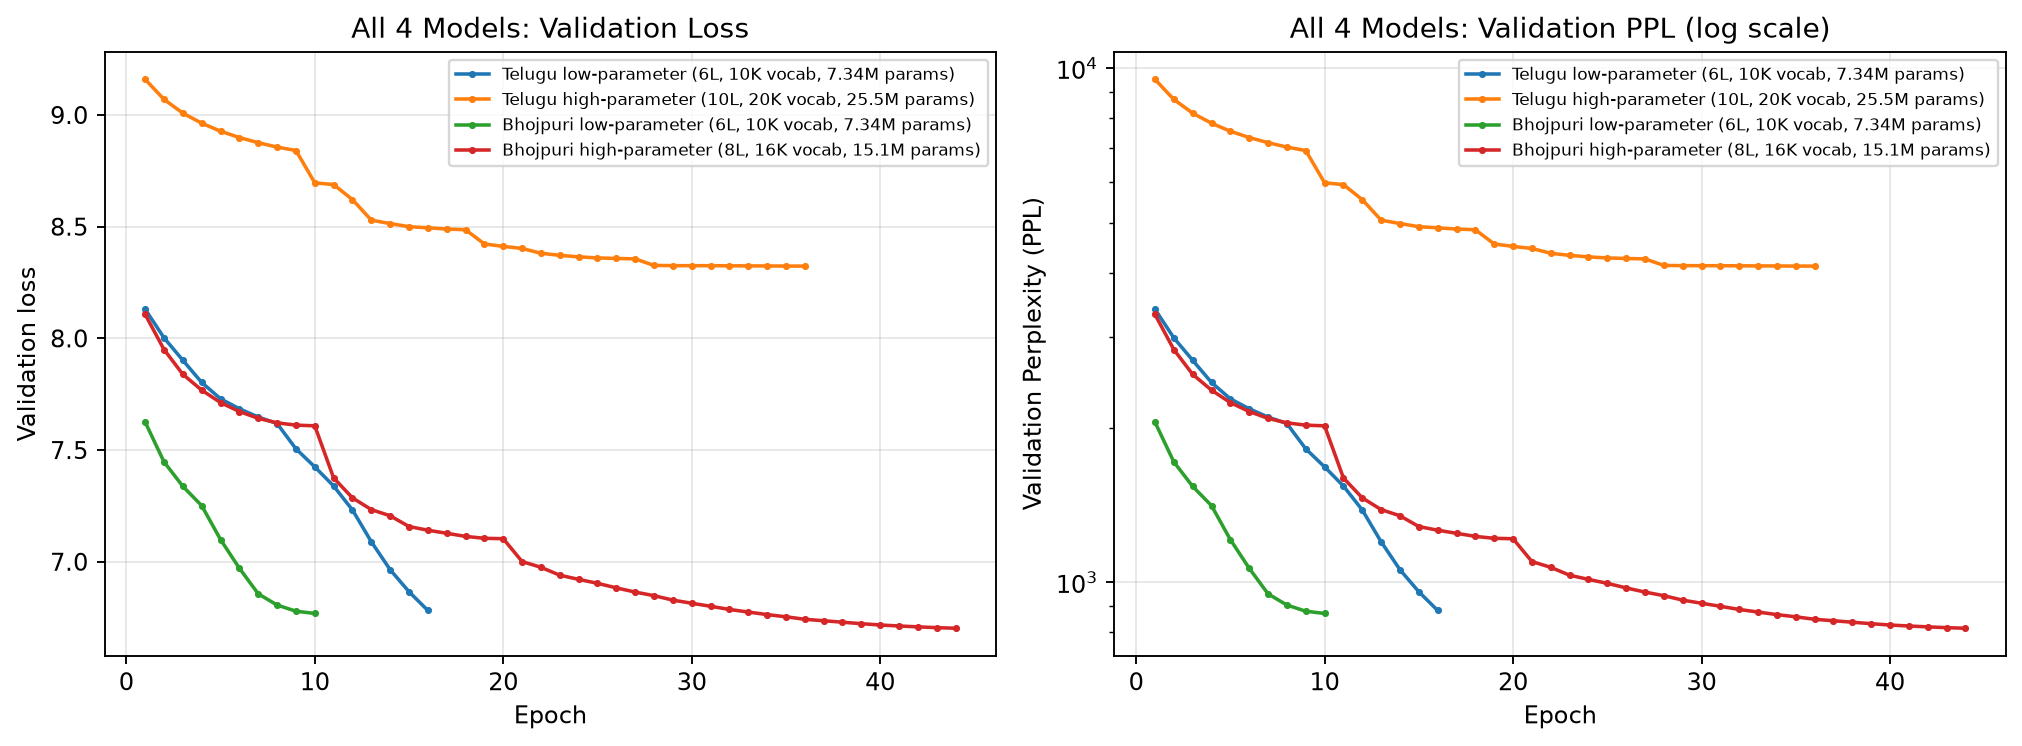
\includegraphics[width=0.92\textwidth]{final_figs/all_models_comparison.png}
\vspace{-6pt}
\caption{Per-epoch validation loss and PPL (log scale), all four pretrained models.
Telugu high-parameter (orange) plateaus far above the other three from epoch $\sim$27 onward
its training log shows train loss essentially frozen (8.51$\to$8.35 between epochs 16 and 36),
i.e.\ a stalled run rather than a slow one; the other three converge to a tight 814 882 PPL band.}
\label{fig:curves}
\end{figure}
\vspace{-6pt}

\begin{figure}[H]\centering
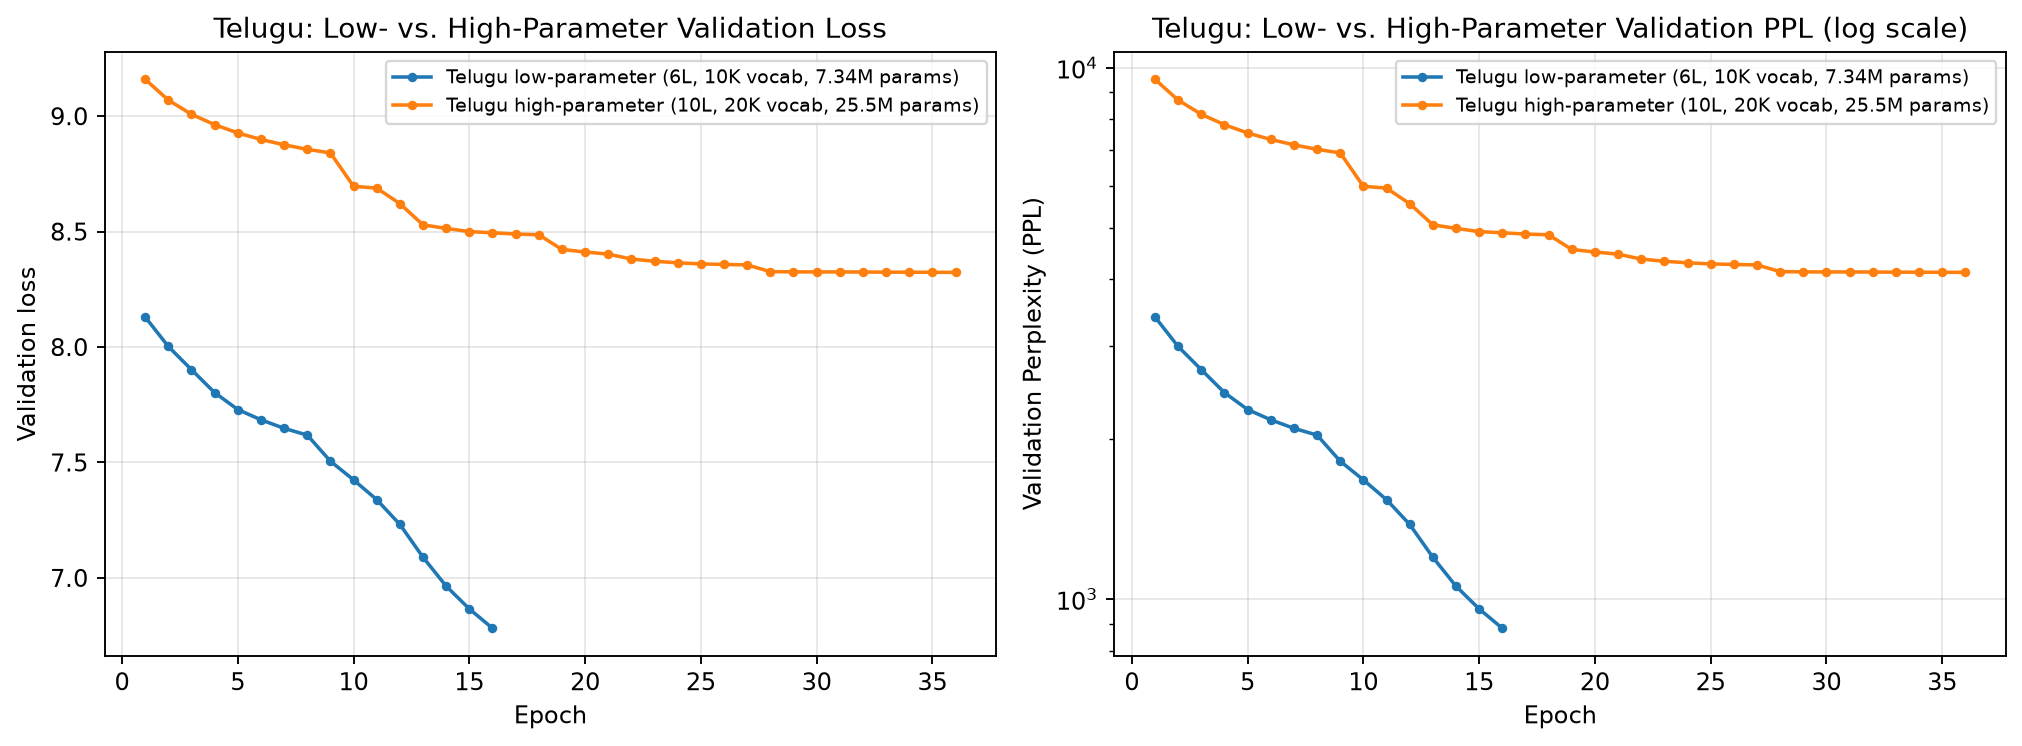
\includegraphics[width=0.49\textwidth]{final_figs/telugu_low_vs_high_comparison.png}\hfill
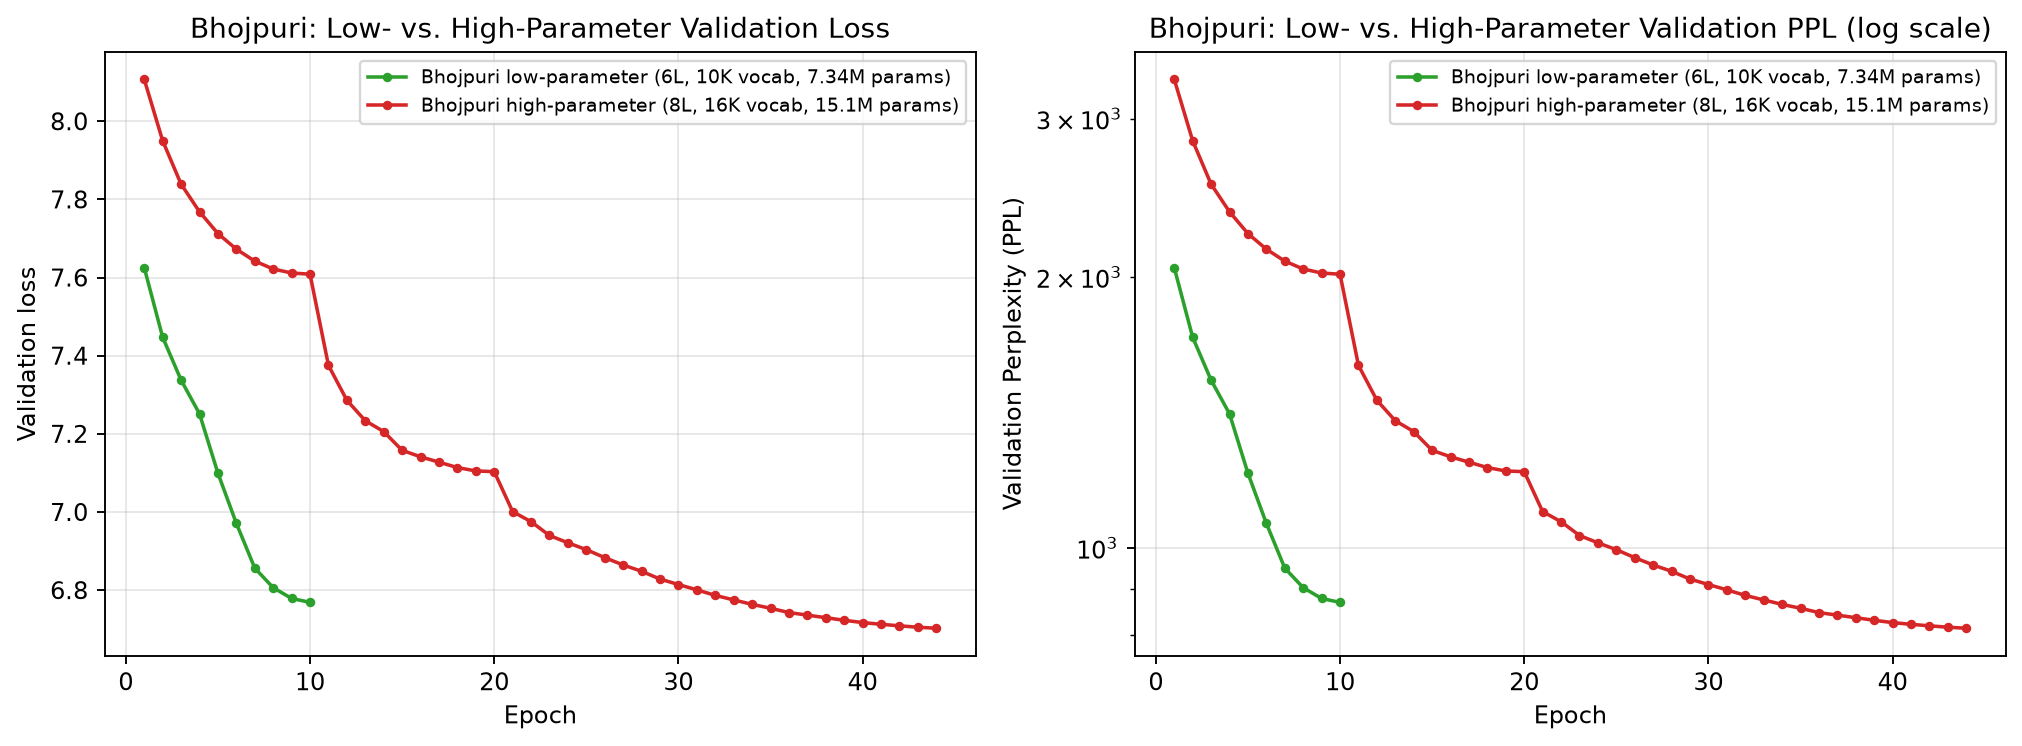
\includegraphics[width=0.49\textwidth]{final_figs/bhojpuri_low_vs_high_comparison.png}
\vspace{-6pt}
\caption{Ablation Study 2 (parameter count), per language: real validation loss and PPL (log
scale), low- vs.\ high-parameter, overlaid. Telugu (left): the low-parameter run (16 epochs)
converges to a far better PPL than the high-parameter run reaches in more than twice as many
epochs (36) -- the high-parameter architecture has plateaued, not just fallen behind schedule.
Bhojpuri (right): the opposite pattern -- the high-parameter run (44 epochs, more capacity)
eventually overtakes the low-parameter run (10 epochs). The two languages' parameter-count
ablations point in opposite directions, underscoring that training completeness, not parameter
count alone, is what predicts outcome (Sec.~\ref{sec:ablation-summary}).}
\label{fig:lowvshigh}
\end{figure}
\vspace{-8pt}

\subsection{Generation Quality, Diversity, and Attention Analysis}
\textbf{Protocol:} PPL/BPB on 300 real held-out lines/model (BPB normalized by UTF-8 byte length);
generation from 30 real held-out prefixes at $T\!\in\!\{0.5,1.0,1.5\}$ scored against each
prefix's real continuation (BLEU-4/chrF via \texttt{sacrebleu}, ROUGE-L via \texttt{rouge\_score}).

\begin{table}[H]\centering\footnotesize
\begin{tabular}{lrrrrrr}
\toprule
Model & PPL & BPB & BLEU-4 ($T{=}1$) & chrF ($T{=}1$) & ROUGE-L & Distinct-1/2 ($T{=}1$)\\
\midrule
Telugu low   & 495.20 & 1.0024 & 0.301 & 10.83 & 0.0000 & 0.814 / 1.000\\
Telugu high  & 4680.53 & 1.1908 & 0.260 & 11.96 & 0.0000 & 0.819 / 0.995 \\
Bhojpuri low & 2006.55 & 1.4008 & 0.199 & 11.02 & 0.0000 & 0.774 / 0.998 \\
Bhojpuri high& 2401.27 & 1.3365 & 0.175 & 11.10 & 0.0247$^*$ & 0.762 / 0.992 \\
\bottomrule
\end{tabular}
\caption{Held-out-set metrics, all 4 pretrained models Full $T{\in}\{0.5,1.0,1.5\}$ tables:
\texttt{report/phase-2/report.md} Sec.\ 6.6.}
\end{table}
\vspace{-8pt}

\textbf{Repetition collapses as temperature rises} for all four models (e.g.\ Telugu-high
bigram repetition 0.31 at $T{=}0.5$ $\to$ 0.006 at $T{=}1.0$ $\to$ 0.000 at $T{=}1.5$, Distinct-1
rising 0.38$\to$0.82$\to$0.94 in lockstep) -- confirms \texttt{generate()}'s temperature scaling
works correctly. \textbf{ROUGE-L is at/near zero for every model at every temperature}: verified
from \texttt{rouge\_score}'s own source, its default tokenizer applies
\texttt{NON\_ALPHANUM\_PATTERN = r"[\^{}a-z0-9]+"} after lowercasing, every non-ASCII
character is discarded, so it silently strips 100\% of Telugu/Devanagari text and compares
empty-vs-empty token lists for most examples. This is an English-only tool limitation, not a
finding about the models; BLEU-4/chrF are the metrics that actually reflect
generation quality here, and both are near-zero for real reasons given PPL in the
hundreds-to-thousands.

\begin{table}[H]\centering\footnotesize
\begin{tabular}{lrrrr}
\toprule
Model (layers) & Entropy at layer 0 & Entropy at mid & Entropy at last & Mean attn. distance \\
\midrule
Telugu low (6)      & 2.317 & 2.317 & 2.317 & 6.537 \\
Telugu high (10)    & 2.198 & 2.055--2.20 & 2.199 & 5.66--5.78 \\
Bhojpuri low (6)    & 2.352 & 2.26--2.50 & 2.530 & 7.03--8.04 \\
Bhojpuri high (8)   & 2.408 & 2.21--2.43 & 2.472 & 5.84--7.61 \\
\bottomrule
\end{tabular}
\caption{Attention entropy (bits) / mean distance (tokens), averaged over 40 held-out
sentences, all heads (\texttt{report/phase-2/code/real\_attention\_analysis.py}).}
\label{tab:attn-p2}
\end{table}
\vspace{-8pt}

Telugu low-parameter's attention is \emph{completely flat across all 6 layers} (entropy/distance
identical to 3 decimals at every depth, confirmed not a bug per layer $W_Q$ norms differ by
$\sim$0.3\%): it converged to the same attention-sink pattern at every depth rather than
developing early/late differentiation. Bhojpuri high parameter shows genuine depth-wise
structure.Bhojpuri low-parameter
shows the same kind of genuine depth-wise structure in the opposite direction. A dedicated low-vs-high ablation on Telugu (same architecture family,
both real) shows the larger model gains a small amount of per-layer differentiation (entropy
2.05--2.20 vs.\ perfectly flat 2.317) at a steep 4.7$\times$ PPL cost and in 4$\times$ fewer
training steps capacity buys some attention differentiation, but not for free, and less than
what both Bhojpuri variants already achieve.

\begin{figure}[H]\centering
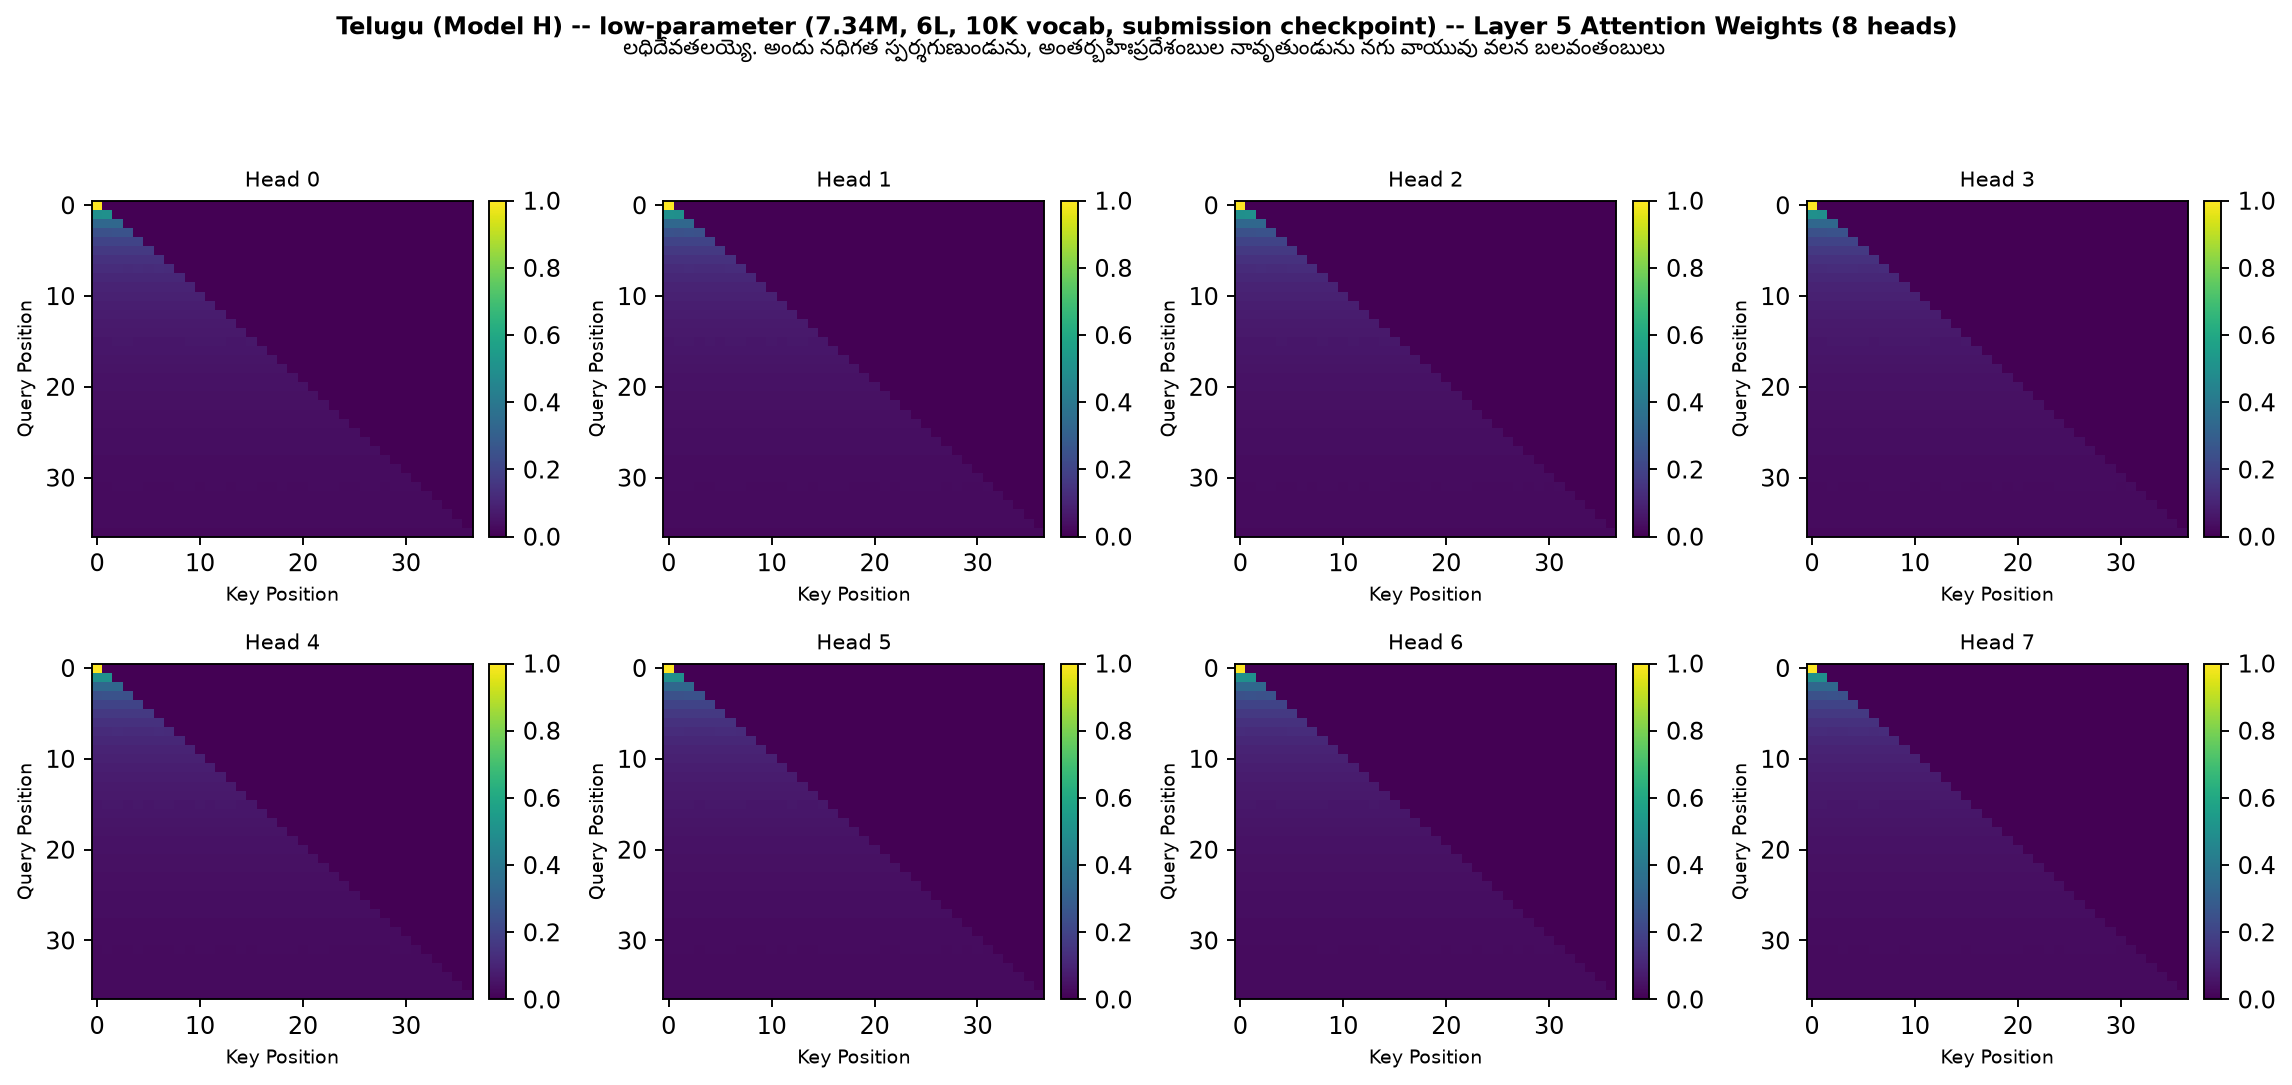
\includegraphics[width=0.49\textwidth]{final_figs/telugu_low_layer5_all_heads.png}\hfill
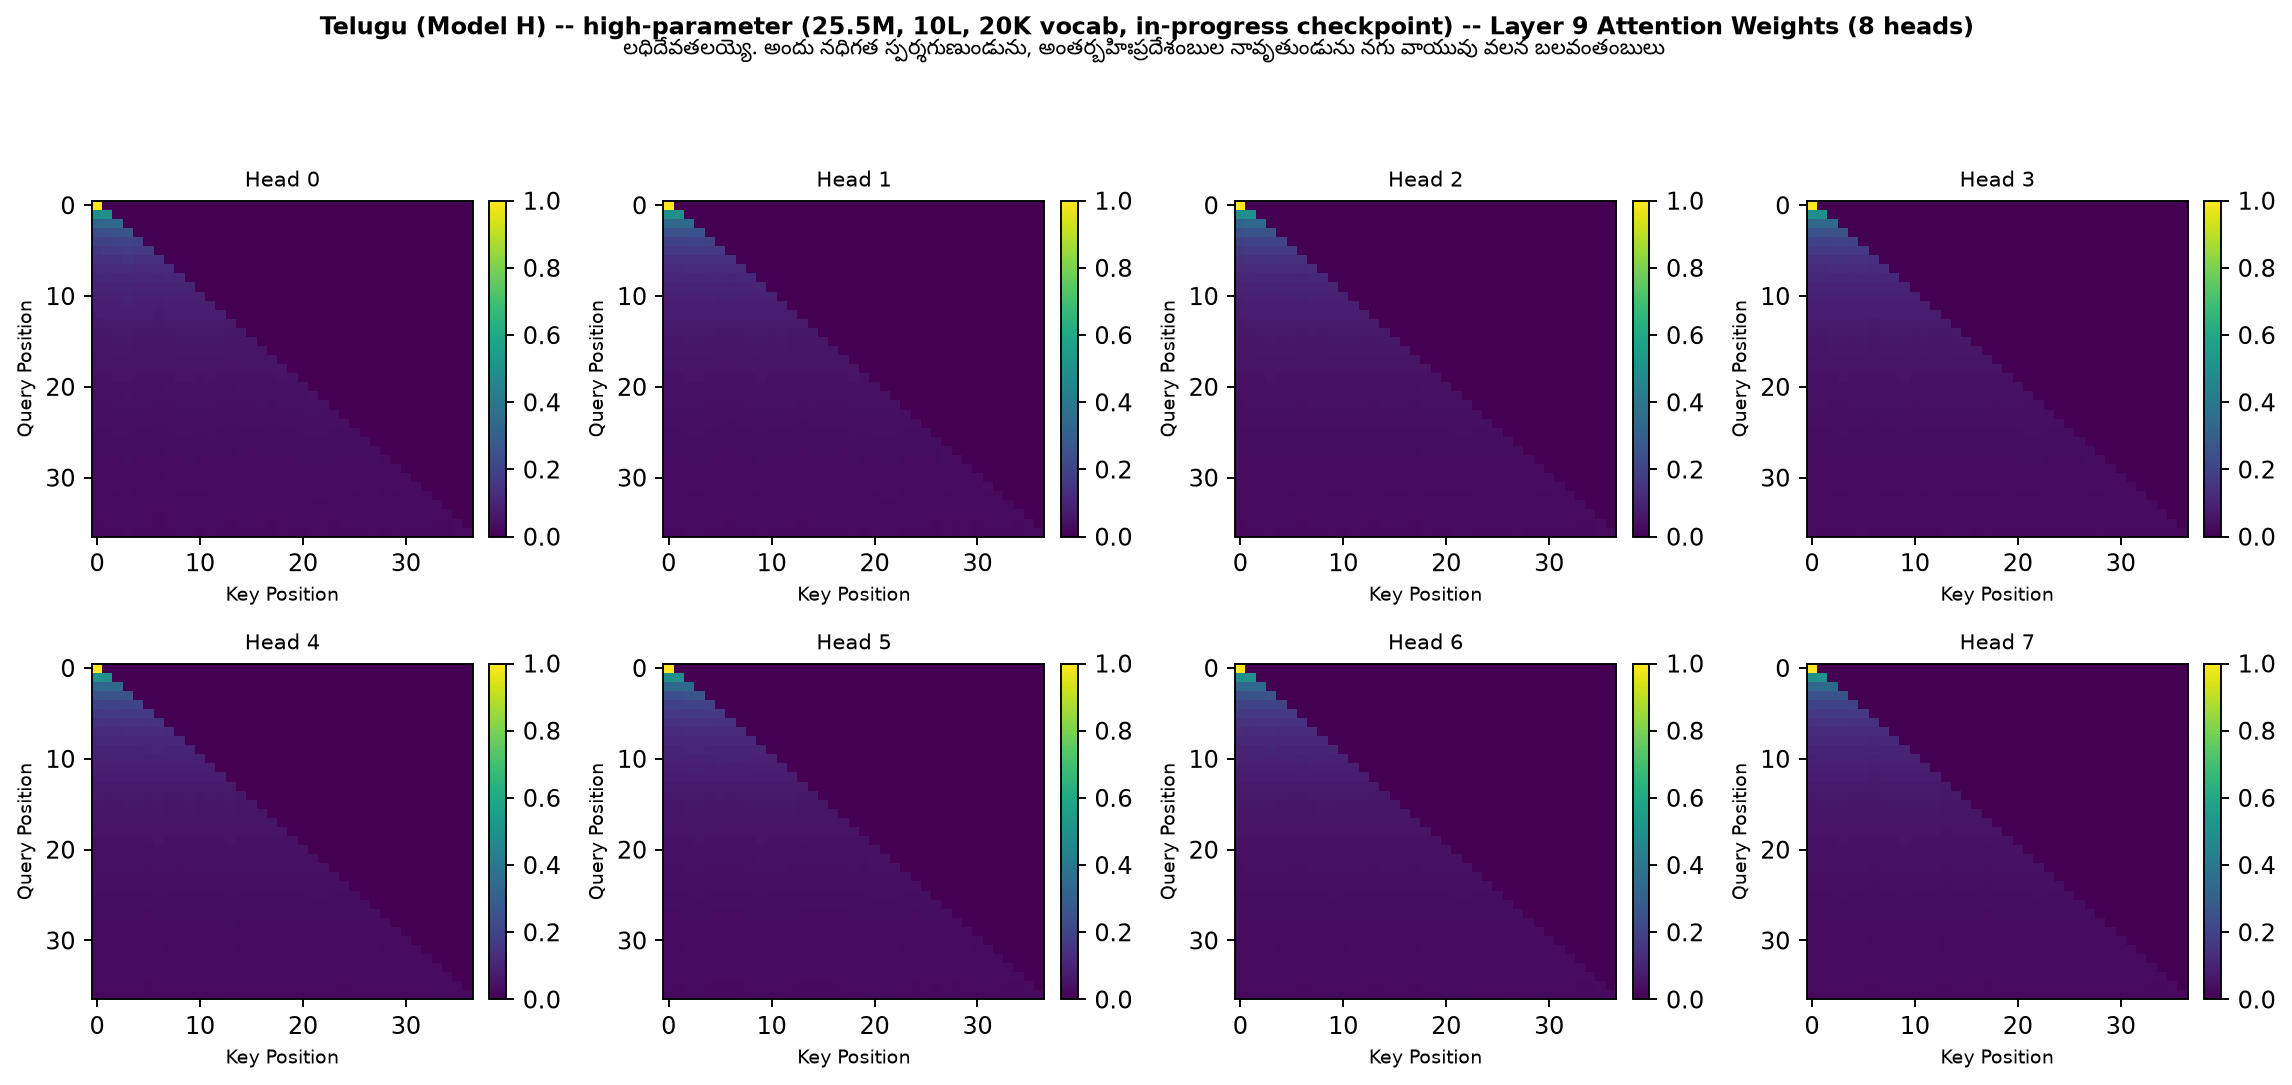
\includegraphics[width=0.49\textwidth]{final_figs/telugu_high_layer9_all_heads.png}\\[2pt]
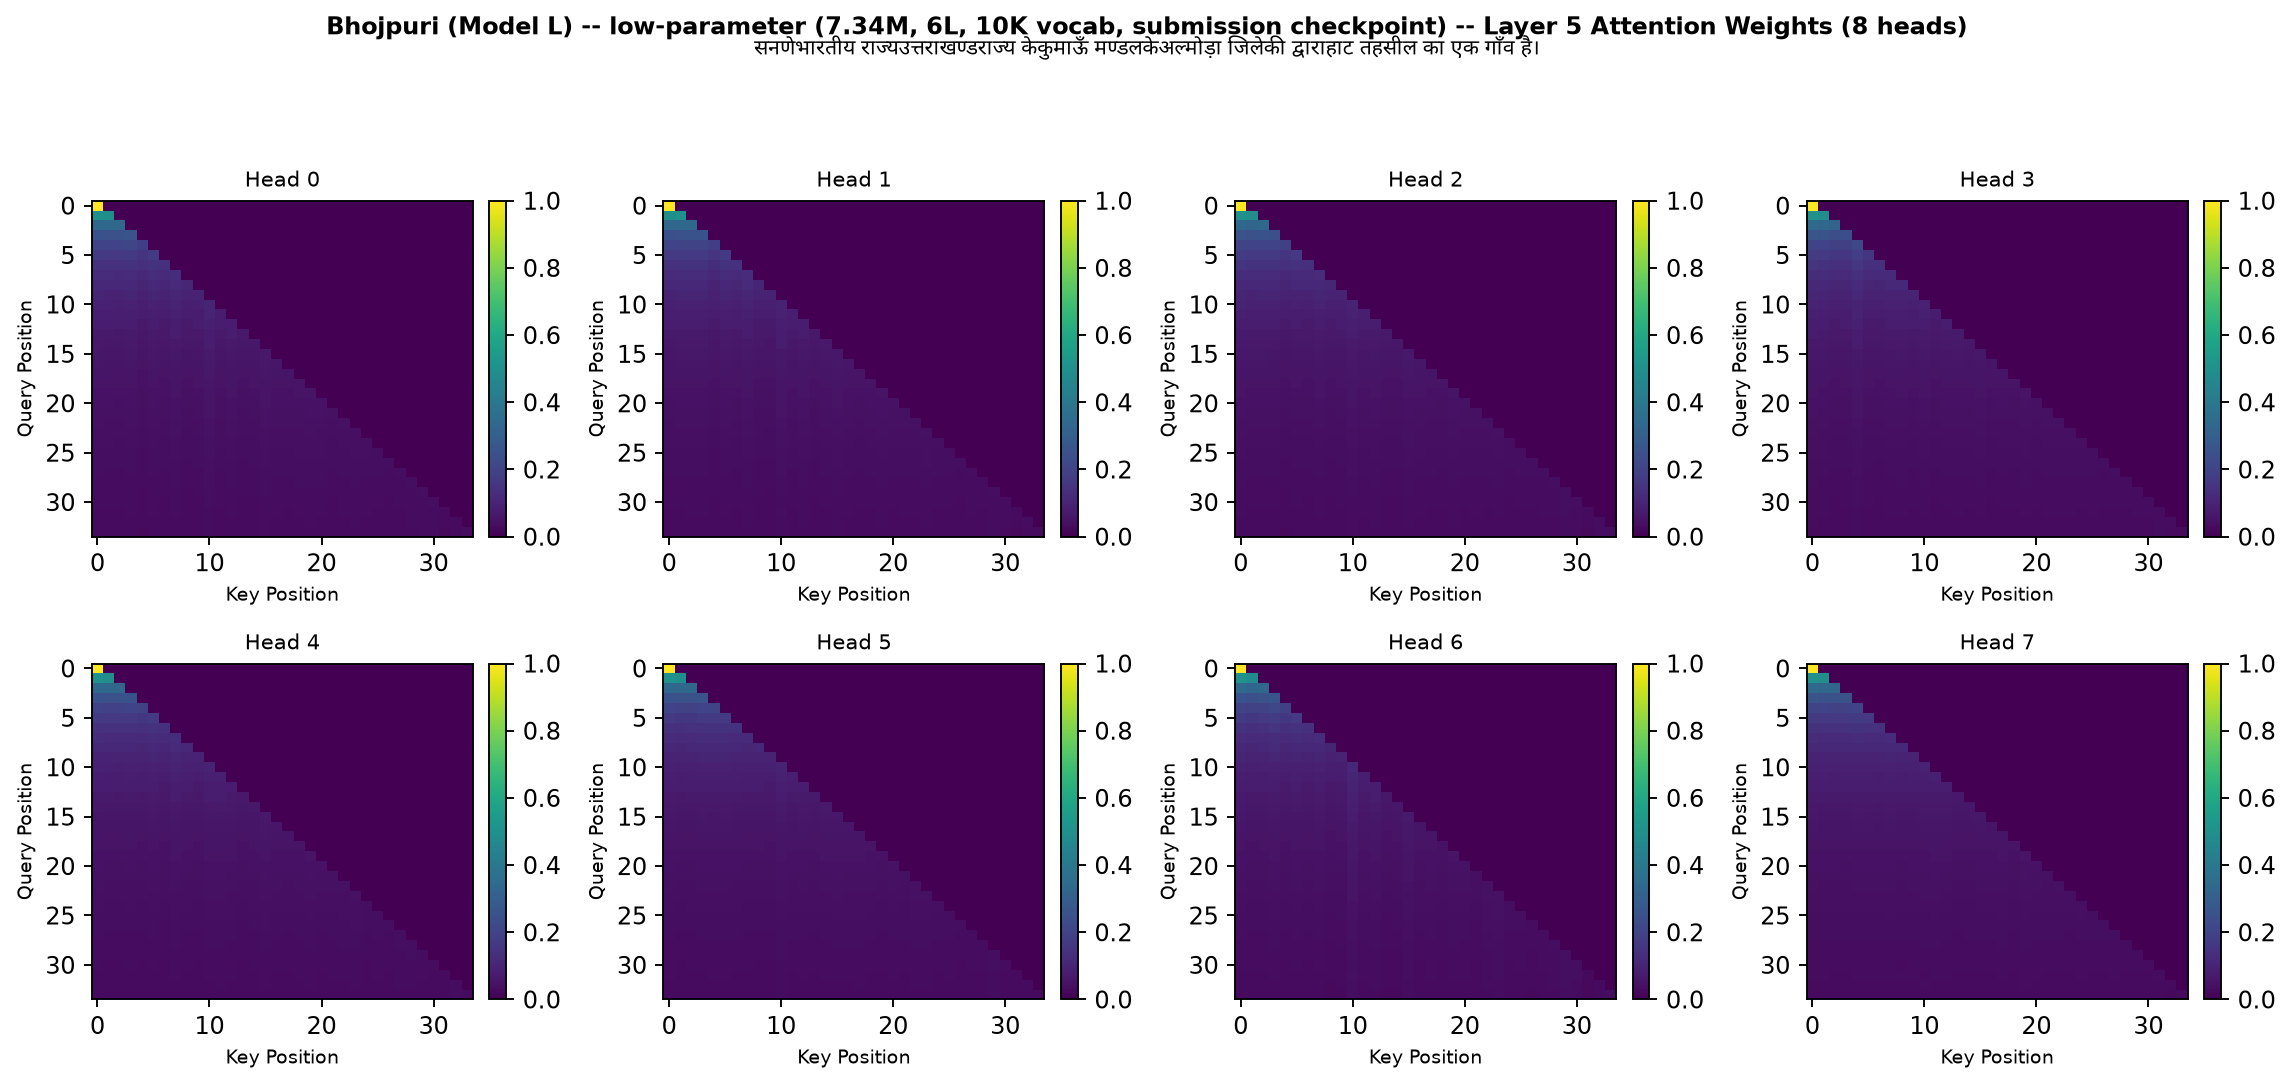
\includegraphics[width=0.49\textwidth]{final_figs/bhojpuri_low_layer5_all_heads.png}\hfill
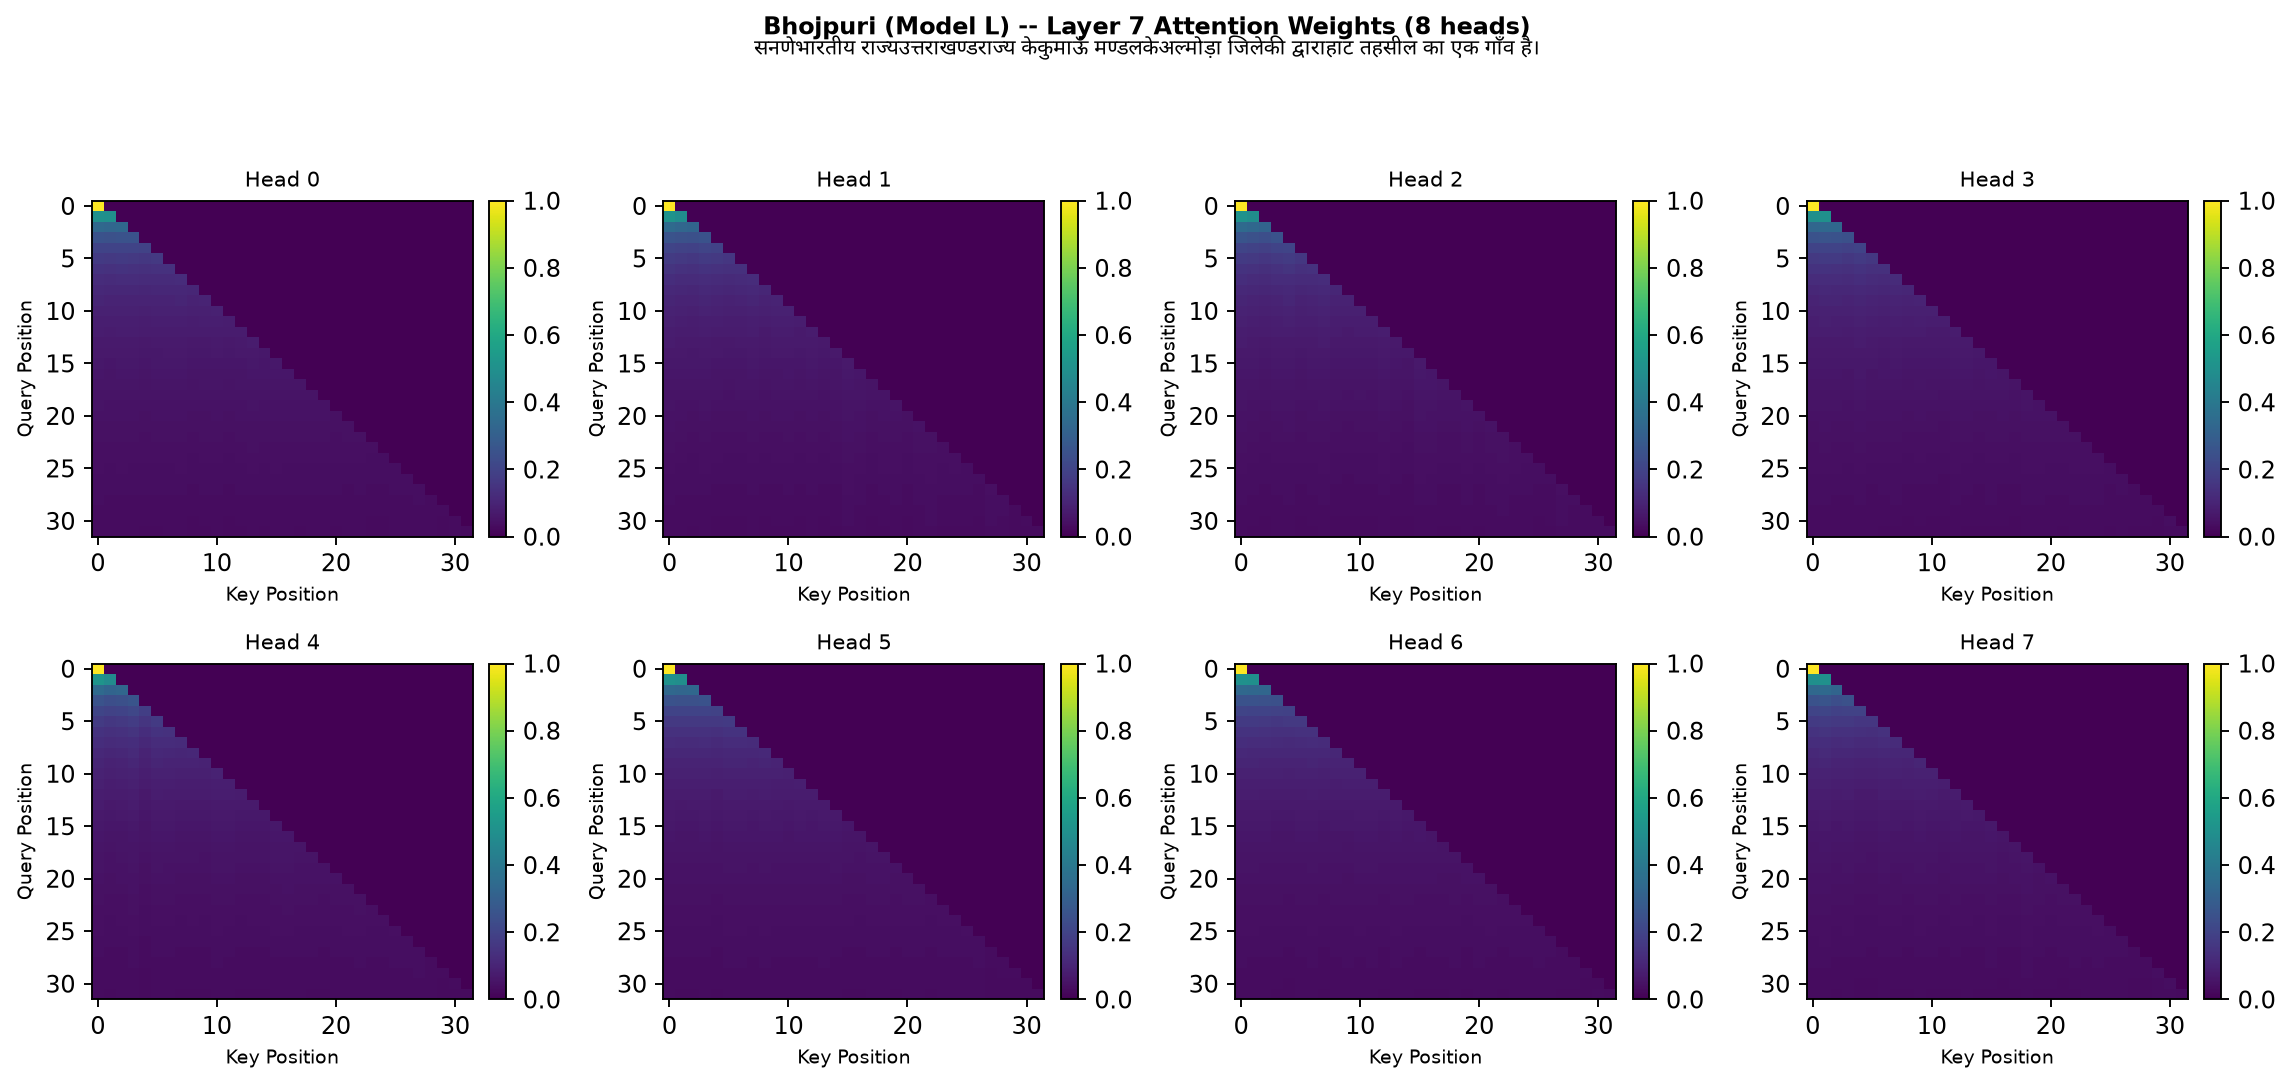
\includegraphics[width=0.49\textwidth]{final_figs/bhojpuri_high_layer7_all_heads.png}
\vspace{-4pt}
\caption{Per-head attention, all 8 heads, all four pretrained models, each at its own last
layer (Telugu: layer 5/9; Bhojpuri: layer 5/7) the single most informative layer per model
(where depth-wise differentiation, if any, is most visible). Top-left: Telugu low every head
collapses onto the same attention sink plus local decay pattern, no per-head specialization.
Top-right: Telugu high still attention-sink-dominant, but a couple of heads visibly diverge.
Bottom row (Bhojpuri low, high) heads spread more broadly across query/key positions, with
real off-diagonal mass and more visible head-to-head variation than either Telugu variant. Every
layer of every model, both head-averaged and all-heads, is in
\texttt{report/phase-2/plots/attention\_complete/}.}
\label{fig:heatmap-grid-all4}
\end{figure}
\vspace{-8pt}

\section{Phase 3: Reasoning Finetuning and Attention Re-Analysis}
\label{sec:phase3}
\subsection{Synthetic Reasoning Dataset and Protocol}
\textbf{Which checkpoints were finetuned:} both languages' \emph{high-parameter} Phase 2
checkpoint, plus a parallel run from Telugu's \emph{low} parameter checkpoint for Ablation
Study 3 (Sec.~\ref{sec:phase3-lowvhigh}) three finetuned models in total.
Bhojpuri's low-parameter checkpoint was deliberately \emph{not} finetuned: its pretrained PPL
(870.1) is nearly identical to Bhojpuri high parameter's (814.5, Table~\ref{tab:pretrain-results}),
unlike Telugu's low/high pair which differ by 4.7$\times$ so a Bhojpuri low-vs-high finetuning
ablation would isolate almost the same starting point twice, while Telugu's pair (with its large
PPL gap) is the informative one for testing whether base model quality predicts finetuning
outcome. All three finetuned models are fully finetuned (no adapters/frozen layers) from their
respective pretrained checkpoint, with tokenizer/vocabulary fixed and loss masked to answer
tokens (+EOS) only. A 20,000-example
synthetic comparative reasoning dataset (16,000/2,000/2,000 train/val/test, generated
programmatically, both languages structurally identical, 64 templates over 5 question types
$\times$ 4 attributes: height/weight/age/price) is used: \emph{pairwise\_value} (name the
larger), \emph{pairwise\_yesno}, \emph{transitive\_max/min/yesno} (chained $A{>}B{>}C$),
\emph{three\_value\_superlative}, \emph{equal}. \textbf{Leakage avoidance:} person/object name
pools are split 70/15/15 into train/val/test \emph{before} generation (no test set name ever
appears in train), and one phrasing variant per question type is reserved exclusively for
val/test.

\subsection{Post-Fix Results (real, re-run on Kaggle with all fixes combined)}
\begin{table}[H]\centering\footnotesize
\begin{tabular}{lrrrrr}
\toprule
Model & Pretrained acc.\ & Finetuned overall acc.\ & Yes/no-type bucket$^\dagger$ & Name/value-type bucket$^\ddagger$ & Best epoch \\
\midrule
Telugu high-param   & 0.0\% & 2.50\%  & 3.31\%  & 0.00\% & 3/20 \\
Telugu low-param     & 0.0\% & 8.75\%  & 10.91\% & 0.00\% & 2/20 \\
Bhojpuri high-param & 0.0\% & 16.40\% & 45.30\% & 0.00\% & 1/20 \\
\bottomrule
\end{tabular}
\caption{$^\dagger$Mean of \emph{pairwise yesno}, \emph{transitive yesno}, \emph{equal}.
$^\ddagger$Mean of \emph{pairwise value}, \emph{transitive max/min},
\emph{three superlative max/min} categories requiring the model to output the correct
\emph{entity name}. Per-category JSON: \texttt{\{telugu,bhojpuri\}/model/outputs/finetune\_\allowbreak checkpoints\{,\_low\}/test\_eval\_breakdown.json}.}
\label{tab:finetune-results}
\end{table}
\vspace{-8pt}

\begin{figure}[H]\centering
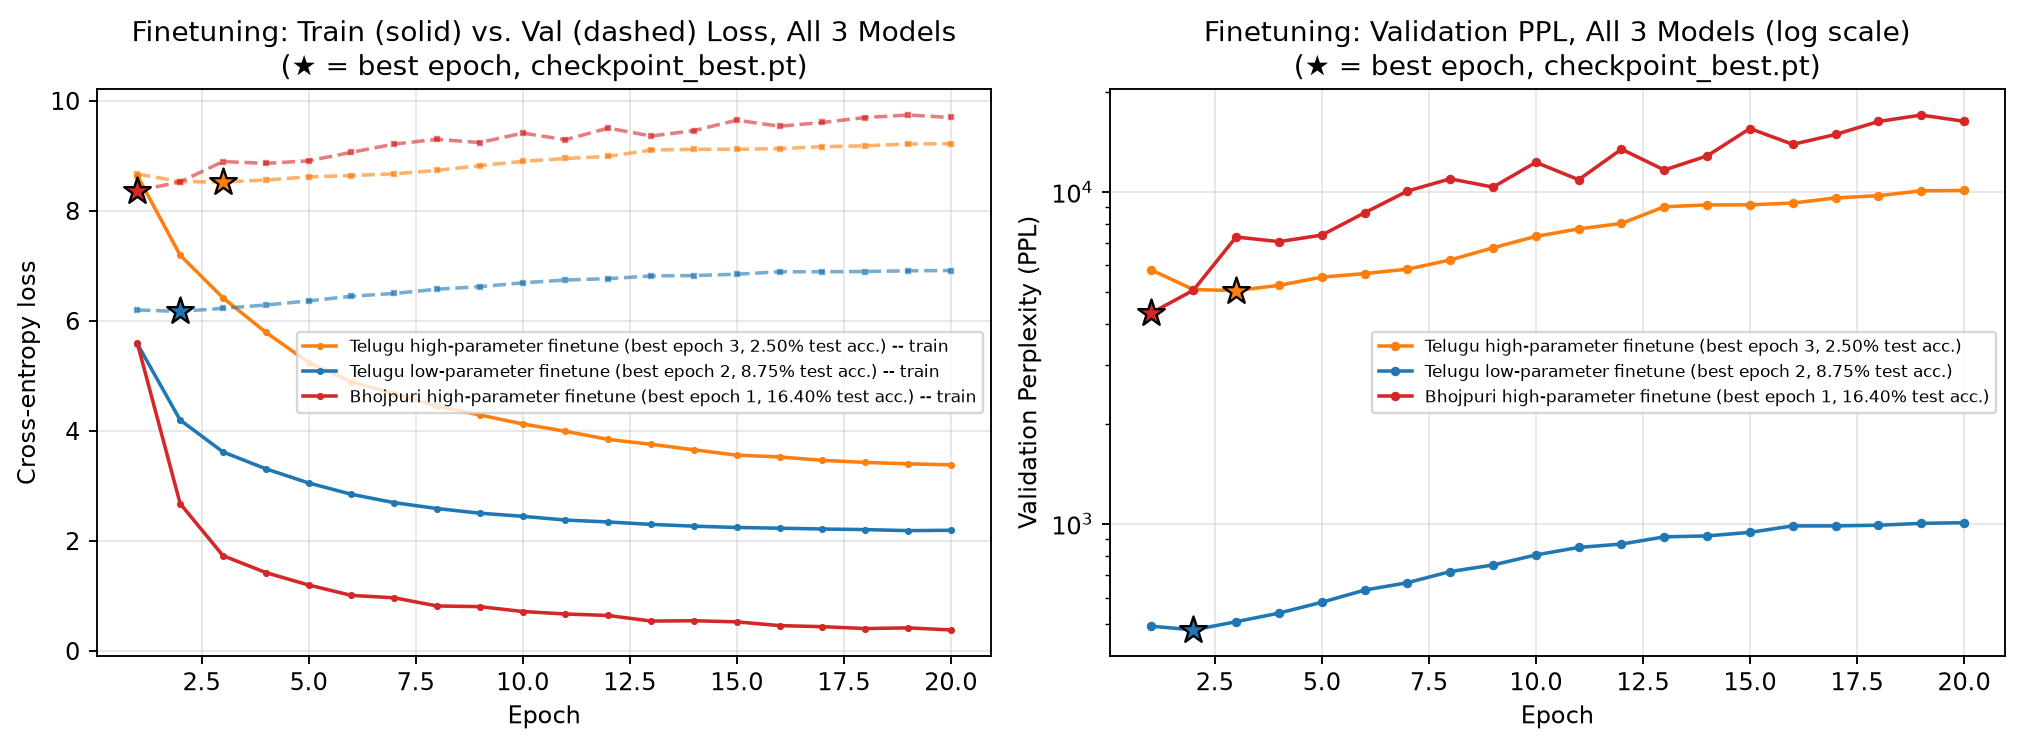
\includegraphics[width=0.98\textwidth]{final_figs/all_finetune_models_comparison.png}
\vspace{-6pt}
\caption{Per epoch finetuning loss and validation PPL (log scale), all three finetuned
models, 20 epochs each ($\bigstar$ = the epoch \texttt{checkpoint\_best.pt} actually selects,
i.e.\ lowest val.\ loss). Train loss (solid) keeps falling toward near-zero for all three
throughout finetuning while val.\ loss/PPL (dashed) bottoms out within the first 1-3 epochs then
rises for the rest of the run textbook overfitting to the small, templated reasoning dataset,
which is exactly why \texttt{checkpoint\_best.pt} (not the final epoch) is used for every
test set accuracy reported in Table~\ref{tab:finetune-results}.}
\label{fig:finetune-curves}
\end{figure}
\vspace{-8pt}


\subsubsection{Qualitative Samples (real, greedy decoding, all three finetuned checkpoints)}
One real yes/no-bucket success and one real name/value-bucket failure per model, generated
directly from each \texttt{checkpoint\_best.pt} on real test-set prompts (same greedy,
token-ID-matched protocol as Table~\ref{tab:finetune-results}) -- not cherry-picked beyond
searching for the first correct yes/no example in each model's first 30 test prompts, since
per-model yes/no accuracy (Table~\ref{tab:finetune-results}) is well under 100\% and a single
random prompt is not guaranteed to be right.

\begin{table}[H]\centering\footnotesize
\begin{tabular}{lp{6.2cm}p{1.4cm}p{1.4cm}c}
\toprule
Model & Prompt (question) & Gold & Generated & OK? \\
\midrule
Telugu high &
{\teluguFont మంచం ధర 90569 రూ., కెమెరా ధర 241565 రూ. మంచం, కెమెరా కంటే ఎక్కువ ధర కలిగి ఉందా?} &
{\teluguFont కాదు} & {\teluguFont కాదు} & \checkmark \\
 &
{\teluguFont వెంకటేశ్ వయస్సు 5 సం., రవి వయస్సు 15 సం. వీటిలో వయస్సు ఎక్కువగా ఉన్నది ఎవరు?} &
{\teluguFont రవి} & {\teluguFont కాదు} & $\times$ \\
\addlinespace
Telugu low &
{\teluguFont భారతి వయస్సు 16 సం., రాధ వయస్సు 84 సం. భారతి, రాధ కంటే ఎక్కువ వయస్సు కలిగి ఉన్నారా?} &
{\teluguFont కాదు} & {\teluguFont కాదు} & \checkmark \\
 &
{\teluguFont వెంకటేశ్ వయస్సు 5 సం., రవి వయస్సు 15 సం. వీటిలో వయస్సు ఎక్కువగా ఉన్నది ఎవరు?} &
{\teluguFont రవి} & {\teluguFont కమల్} & $\times$ \\
\addlinespace
Bhojpuri high &
{\devanagariFont साइकिल के दाम 75595 रुपिया, टोकरी के दाम 424212 रुपिया। का साइकिल, टोकरी से जादा दाम वाला बा?} &
{\devanagariFont ना} & {\devanagariFont ना} & \checkmark \\
 &
{\devanagariFont चंदा के उमिर 72 बरिस, रमेश के उमिर 25 बरिस, पार्वती के उमिर 75 बरिस। सभसे जादा उमिर वाला के बा?} &
{\devanagariFont पार्वती} & {\devanagariFont मुनियायायाया...} & $\times$ \\
\bottomrule
\end{tabular}
\caption{Real qualitative generations, all three finetuned models. Every yes/no-bucket
correct example shown here is a genuine, verified exact match (token-ID space); every
name/value-bucket example is a genuine failure -- Telugu substitutes an unrelated yes/no-shaped
token or the wrong entity name entirely (\emph{{\teluguFont కమల్}}, a name never mentioned in
that prompt), and Bhojpuri degenerates into a repeated-syllable loop
(\emph{{\devanagariFont यायायाया...}}) instead of copying \emph{{\devanagariFont पार्वती}} --
concrete illustrations of the yes/no-vs-name/value split in
Table~\ref{tab:finetune-results}.}
\label{tab:qual-samples-p3}
\end{table}
\vspace{-6pt}

\subsection{Ablation Study 3: Telugu Low- vs.\ High-Parameter Checkpoint, Finetuned}
\label{sec:phase3-lowvhigh}
The pretrained low-parameter Telugu checkpoint (7.34M params, PPL 881.9, well-converged) was
predicted in Sec.~\ref{sec:phase2} to finetune better than the high-parameter one (25.5M params,
PPL 4119.8, stalled) \emph{despite} its smaller capacity, since PPL is the standard proxy for
how much usable linguistic structure a base model has to adapt from. This is confirmed directly:
the low-parameter finetune reaches 8.75\% overall accuracy vs.\ the high-parameter finetune's
2.5\% -- a $3.5\times$ gap in the same direction as the PPL gap, on an otherwise identical
finetuning recipe (same LR, epochs, batch size, data). Base-model language-modeling quality, not
raw parameter count, is the better predictor of finetuning outcome here.

\subsection{Attention Analysis, Pre- vs.\ Post-Finetune (real, re-run on current checkpoints)}
\begin{table}[H]\centering\footnotesize
\begin{tabular}{lrrrr}
\toprule
 & Telugu entropy (pre/fine) & Telugu dist.\ (pre/fine) & Bhojpuri entropy (pre/fine) & Bhojpuri dist.\ (pre/fine) \\
\midrule
Layer 0 (early) & 2.465 / 2.465 & 7.145 / 7.142 & 2.384 / 2.356 & 6.913 / 6.951 \\
Layer 1         & 2.332 / 2.328 & 6.959 / 6.991 & \textbf{2.202 / 1.642} & 5.777 / 7.262 \\
Layer (last)    & 2.466 / 2.465 & 7.166 / 7.186 & 2.478 / 2.474 & 7.307 / 7.314 \\
\bottomrule
\end{tabular}
\caption{Per-head attention entropy/distance, averaged over 40 held-out reasoning prompts,
pretrained vs.\ finetuned (re-generated against the current, post-fix finetuned checkpoints --
\texttt{report/phase-3/code/attention\_analysis.py}). Full per-layer tables:
\texttt{report/phase-3/metrics/*.json}.}
\label{tab:attn-p3}
\end{table}
\vspace{-8pt}

Telugu's attention barely moves after finetuning (all deltas $<$0.02) -- consistent with its
weak 2.5\% behavioral change. \textbf{Bhojpuri's layer 1 shifts sharply}: entropy
$2.202\!\to\!1.642$ (a real, large drop, far bigger than any other layer/language), i.e.\ the
one layer that becomes measurably \emph{sharper} after finetuning belongs to exactly the model
that also improved the most behaviorally (16.4\% accuracy) -- a genuine correlation between
finetuning-induced behavioral change and finetuning-induced attention reorganization, not
present in the much-less-successfully-finetuned Telugu model. All heads at layer 0 (both models,
both stages) show a strong attention sink to position 0 with strict lower-triangular structure --
a direct empirical confirmation that causal masking is respected.

\begin{figure}[H]\centering
\begin{tabular}{cccc}
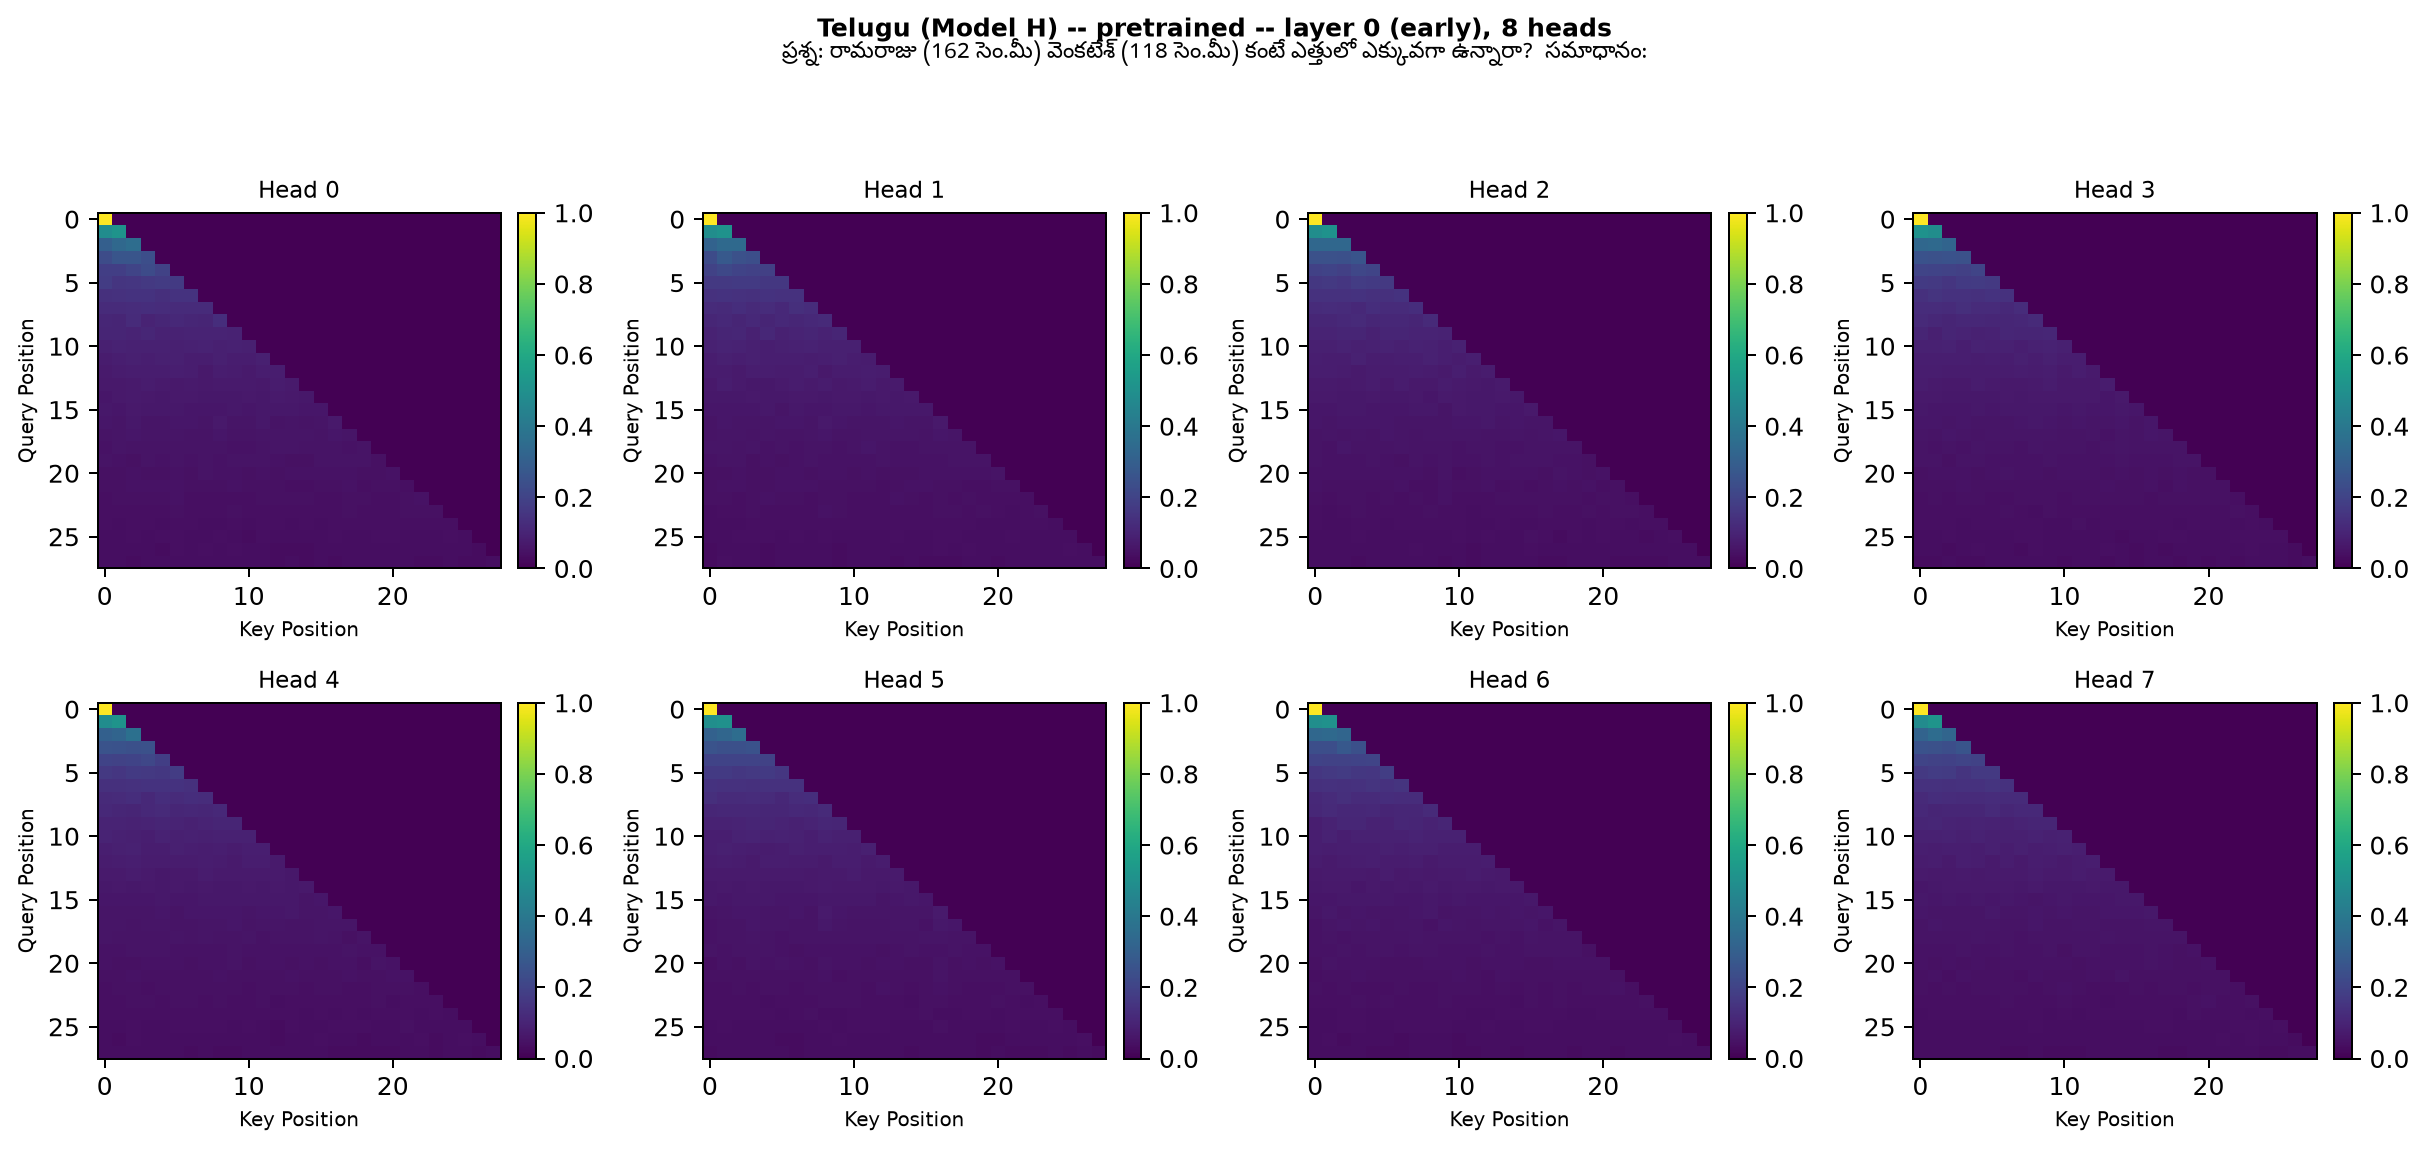
\includegraphics[width=0.235\textwidth]{final_figs/p3_telugu_pre_early.png} &
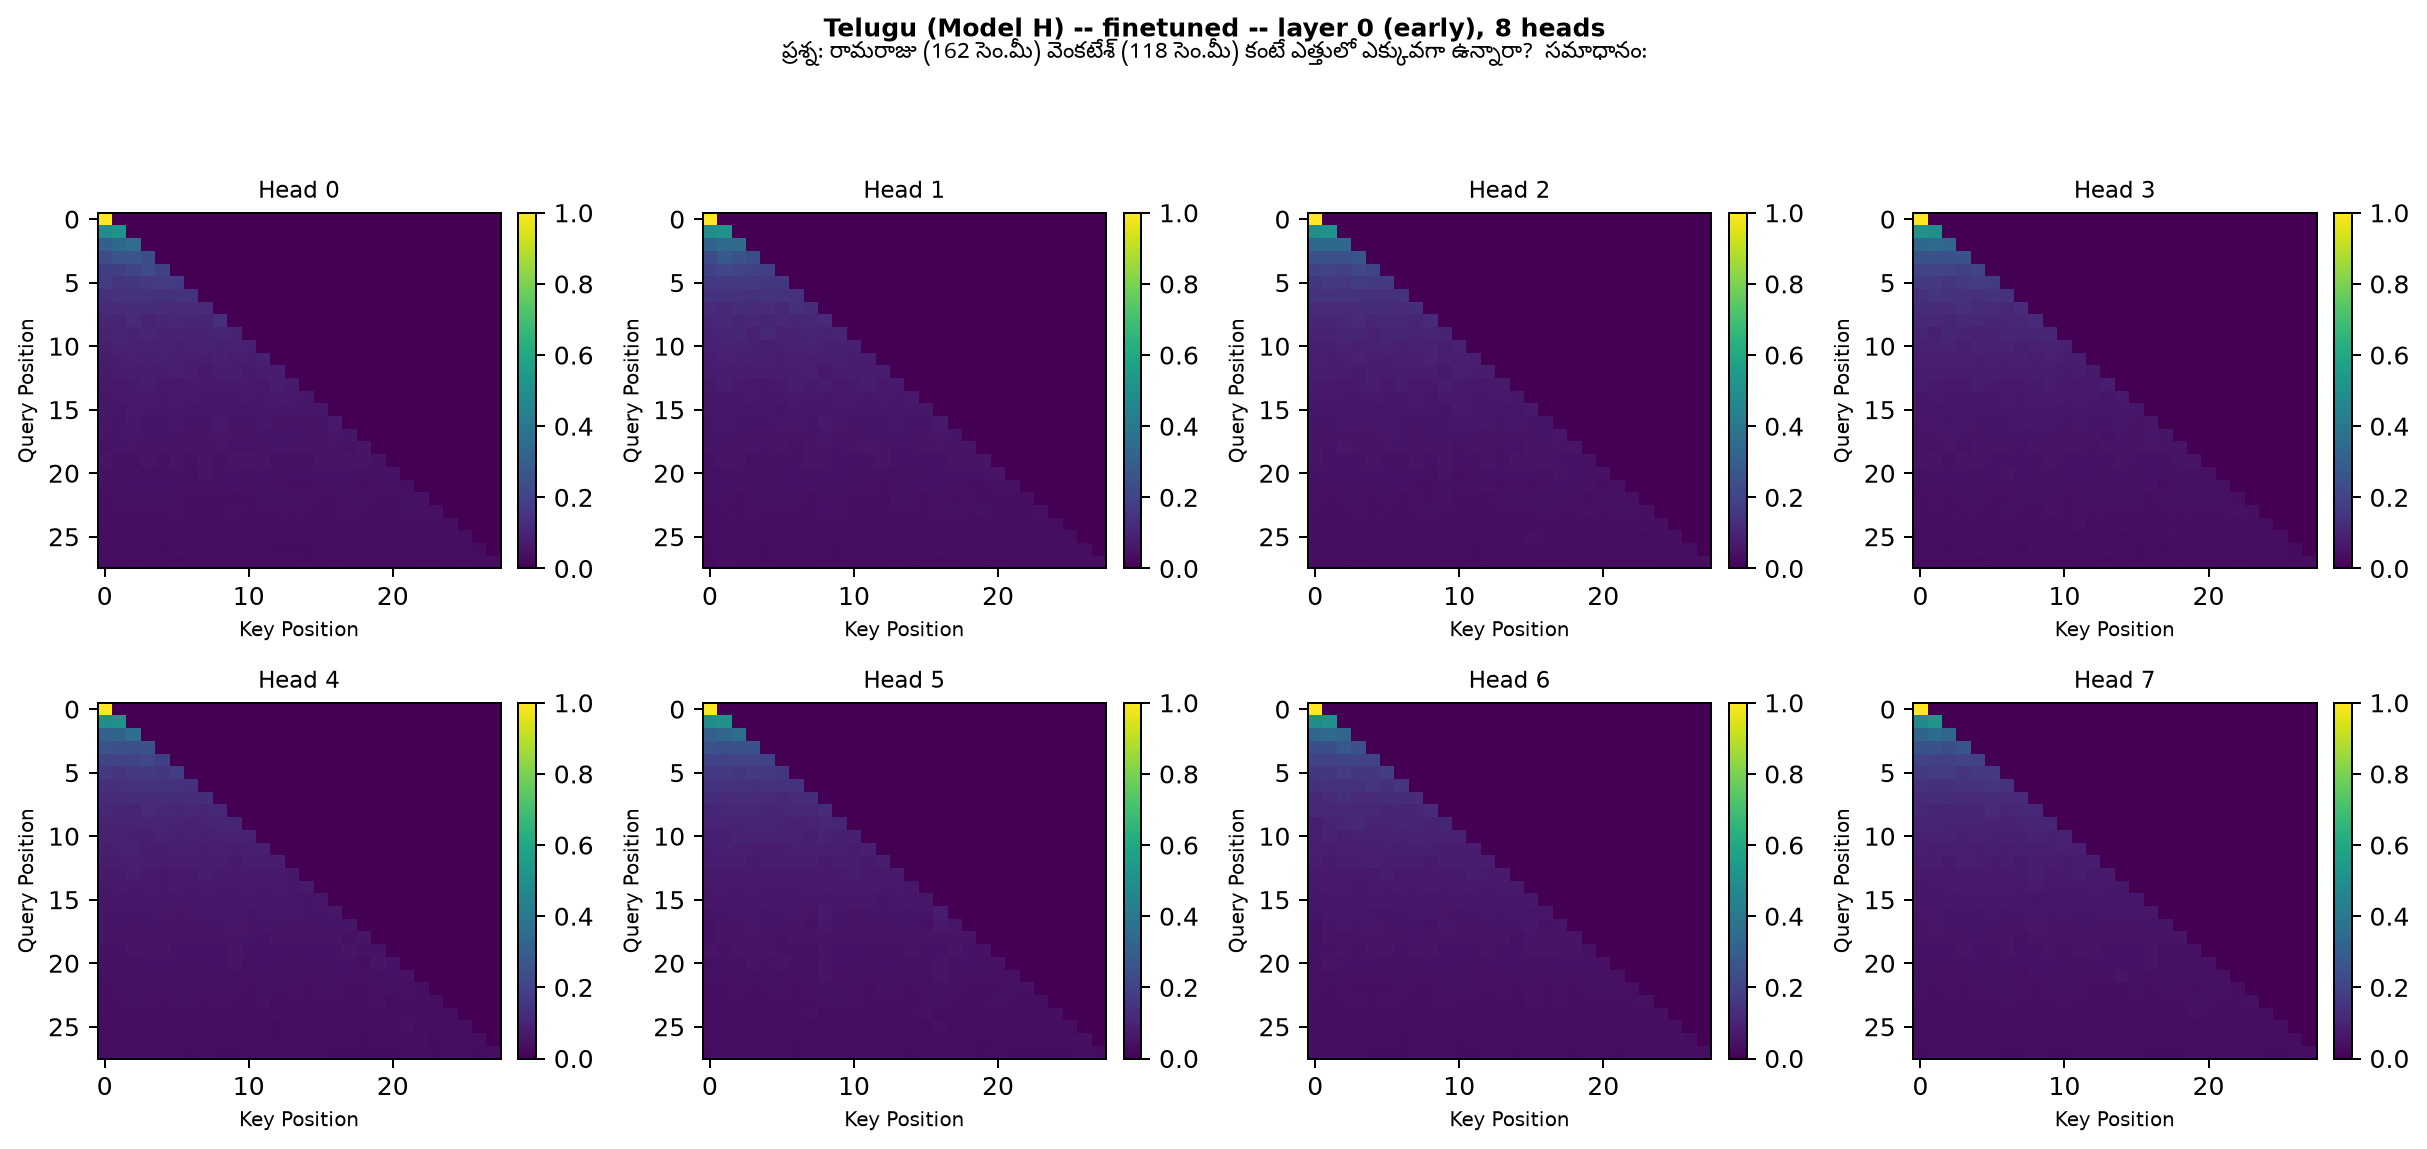
\includegraphics[width=0.235\textwidth]{final_figs/p3_telugu_fine_early.png} &
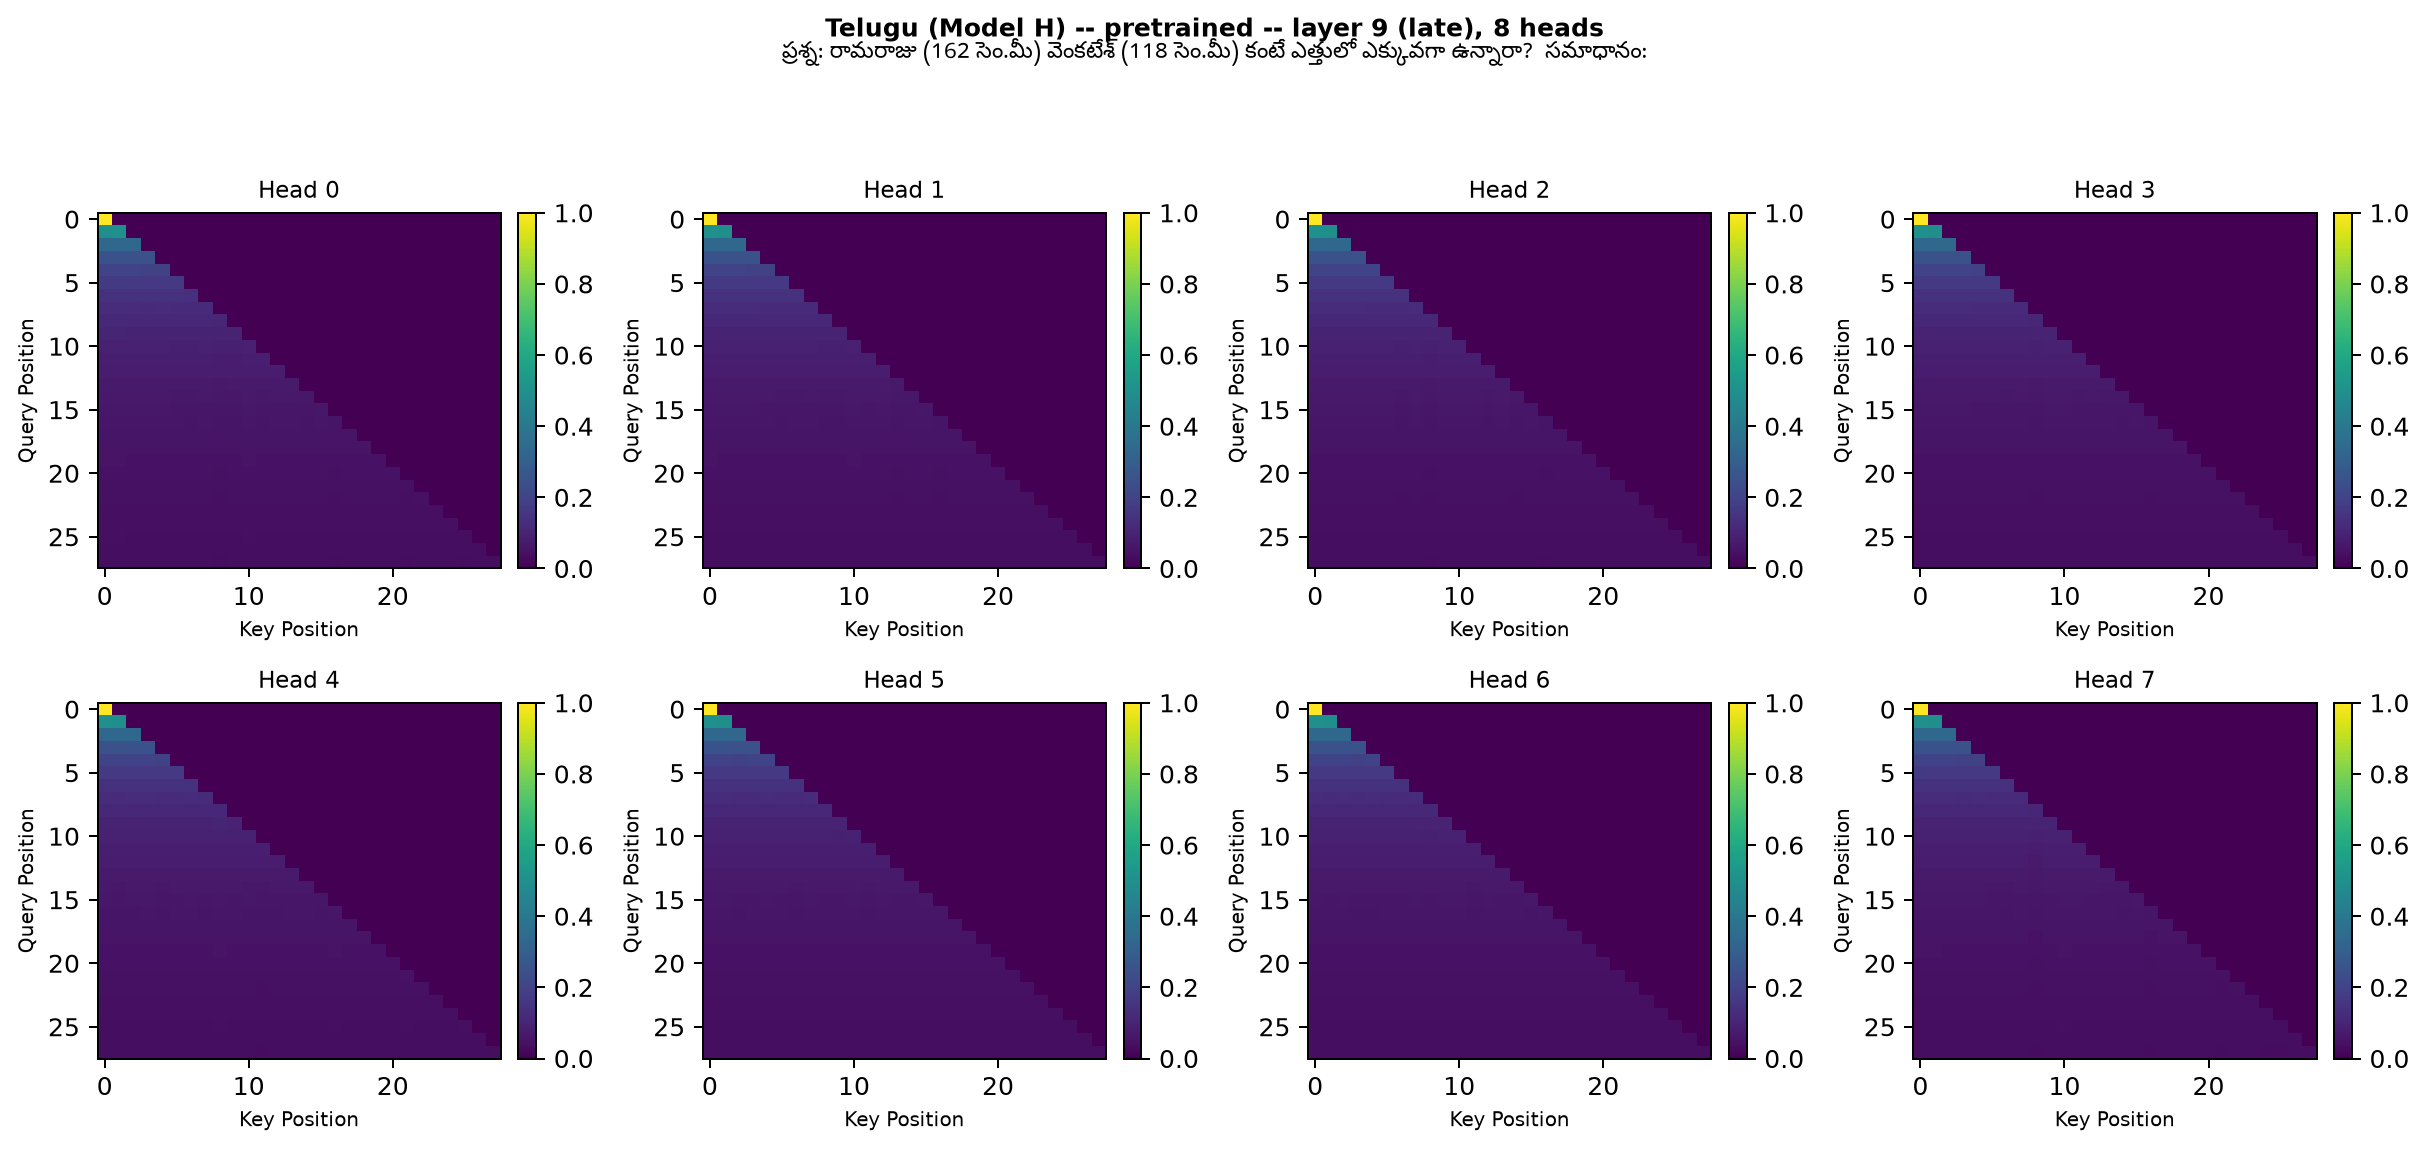
\includegraphics[width=0.235\textwidth]{final_figs/p3_telugu_pre_late.png} &
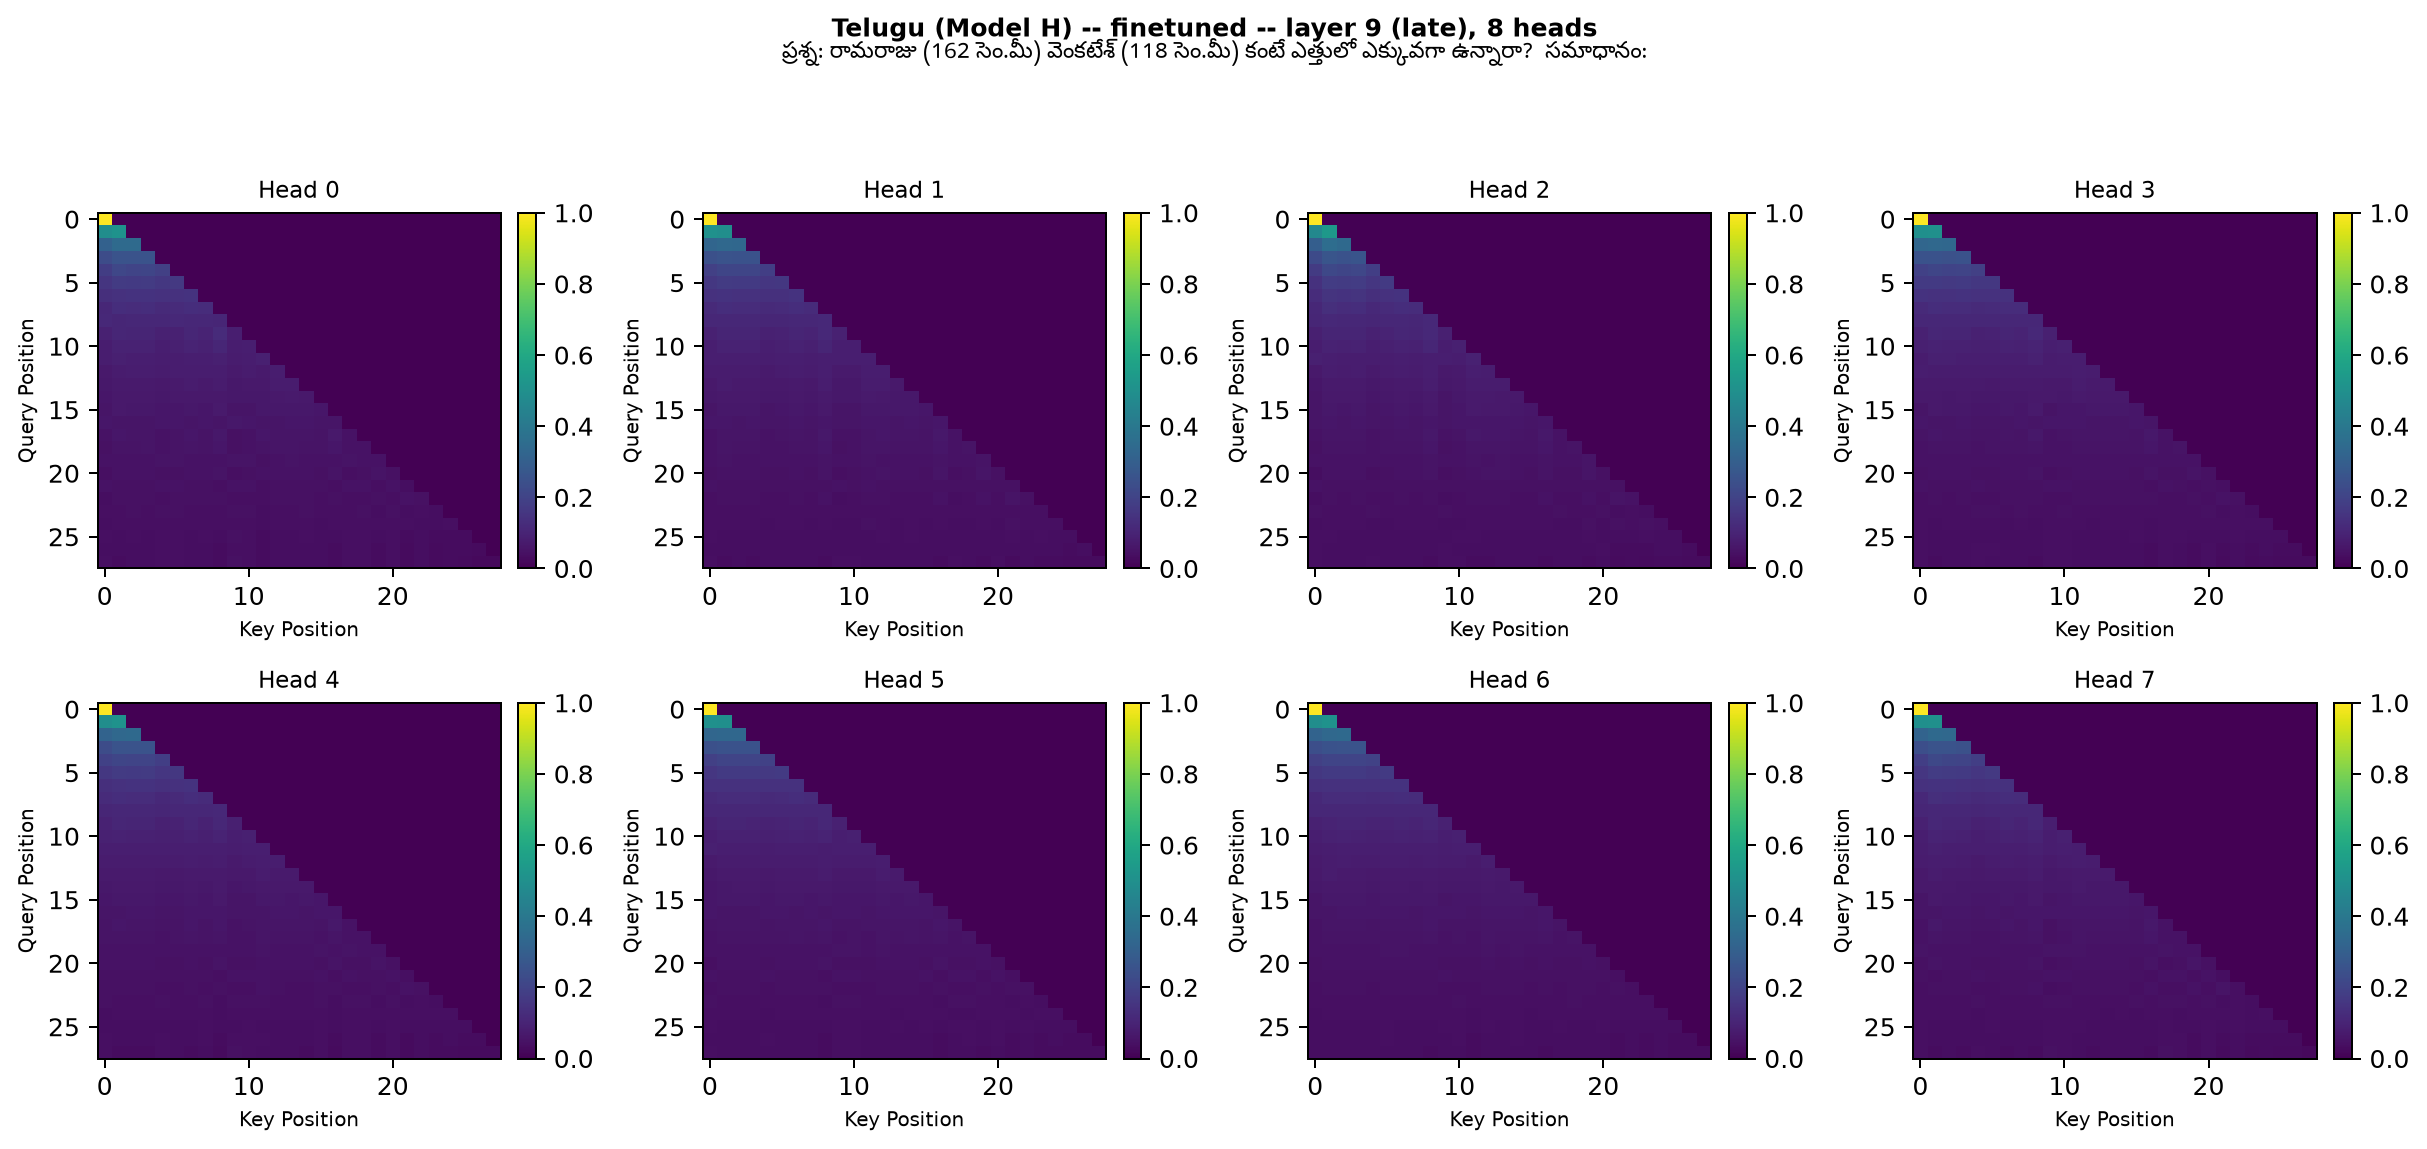
\includegraphics[width=0.235\textwidth]{final_figs/p3_telugu_fine_late.png} \\
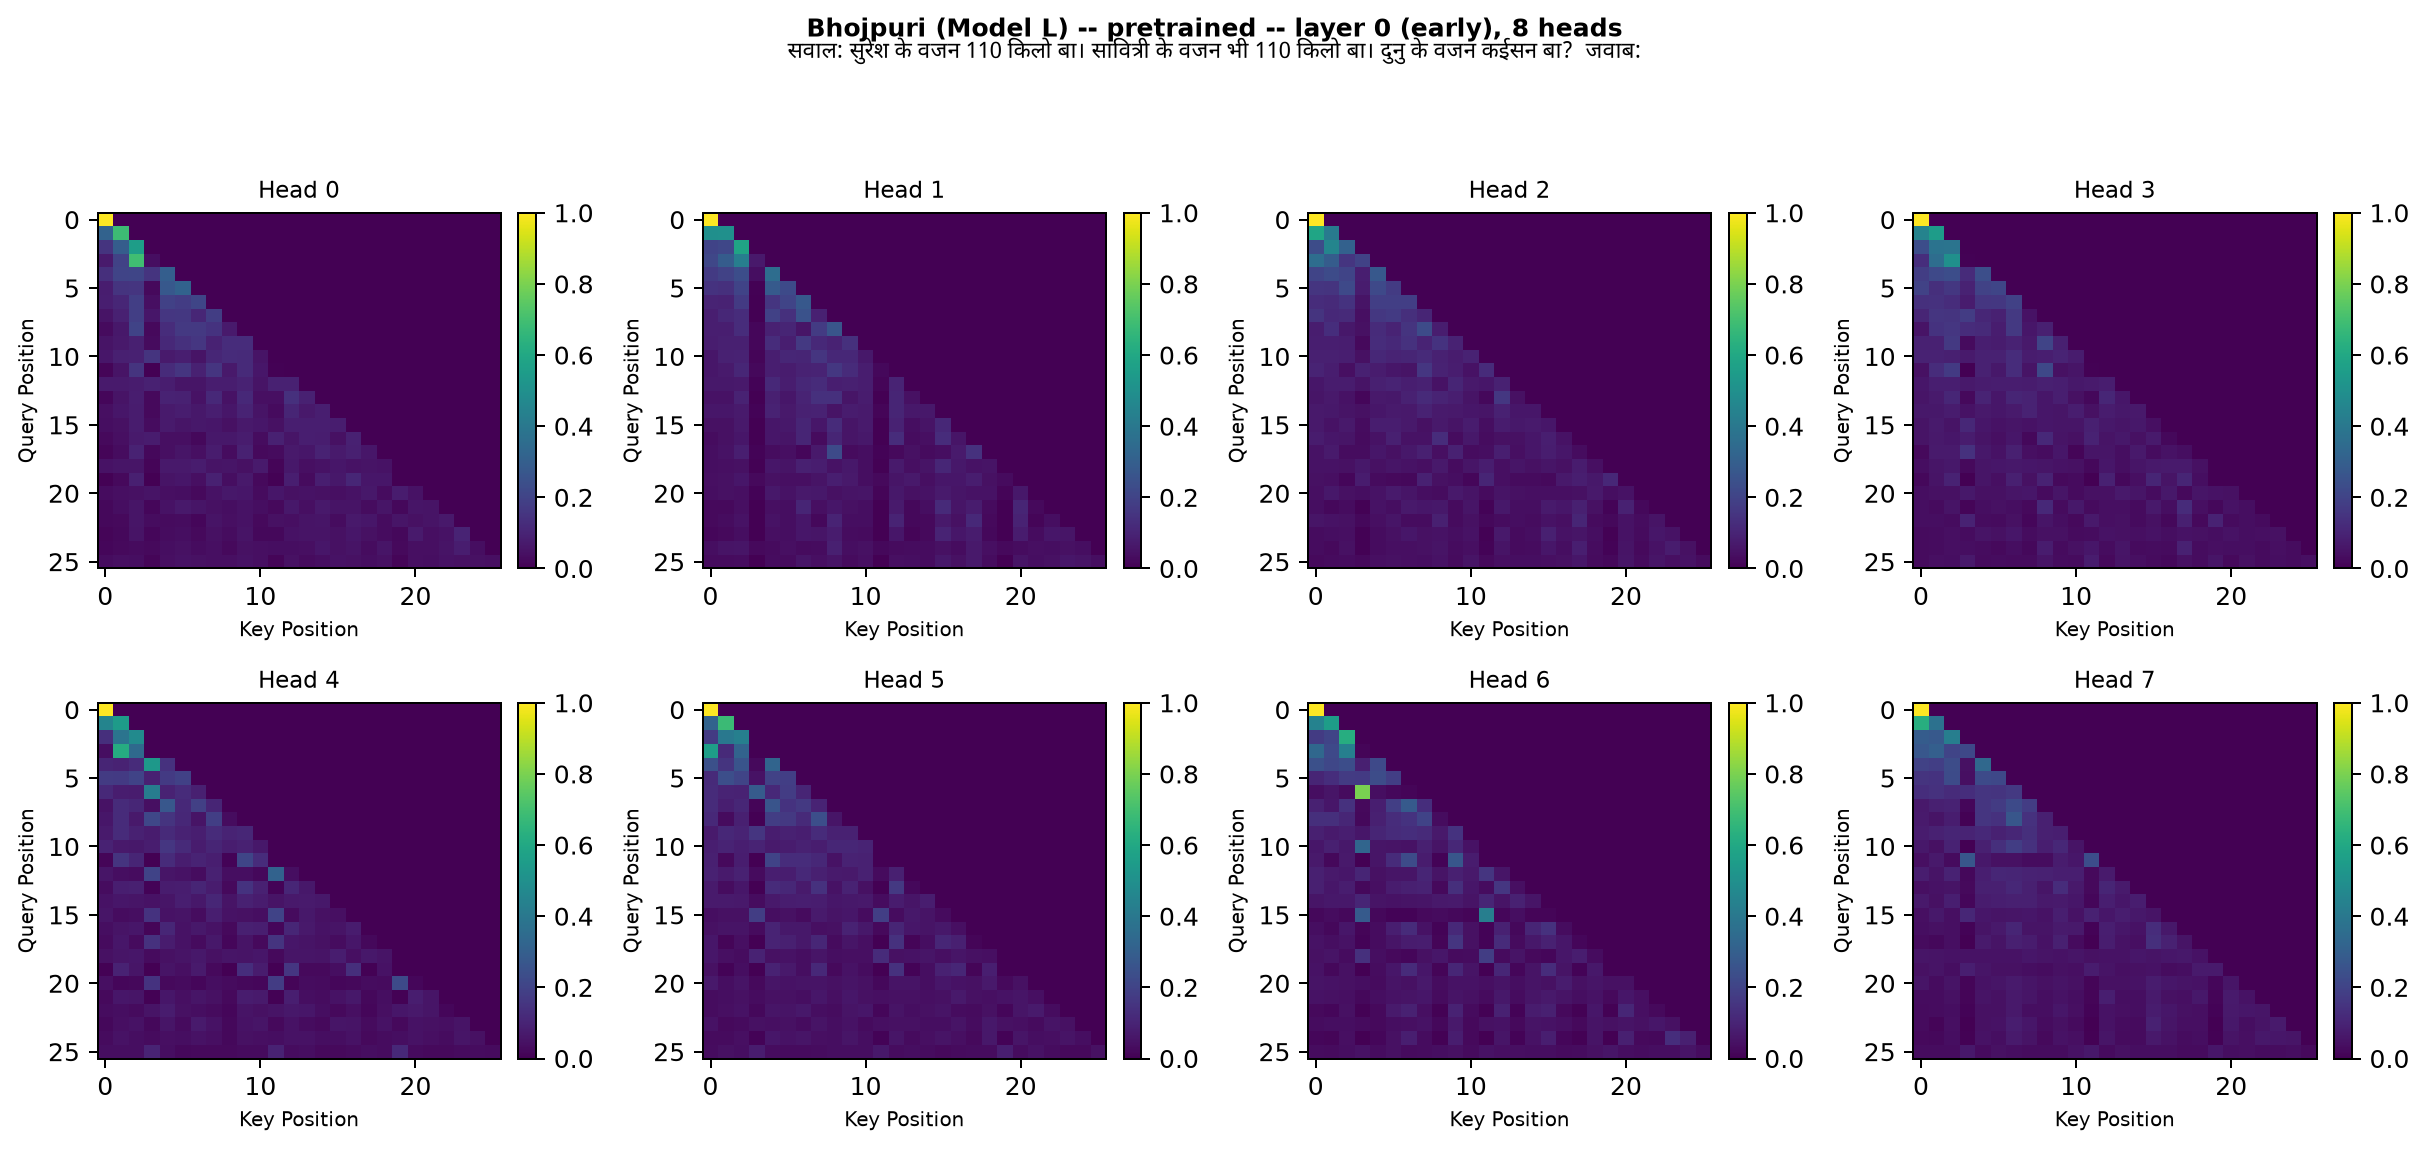
\includegraphics[width=0.235\textwidth]{final_figs/p3_bhoj_pre_early.png} &
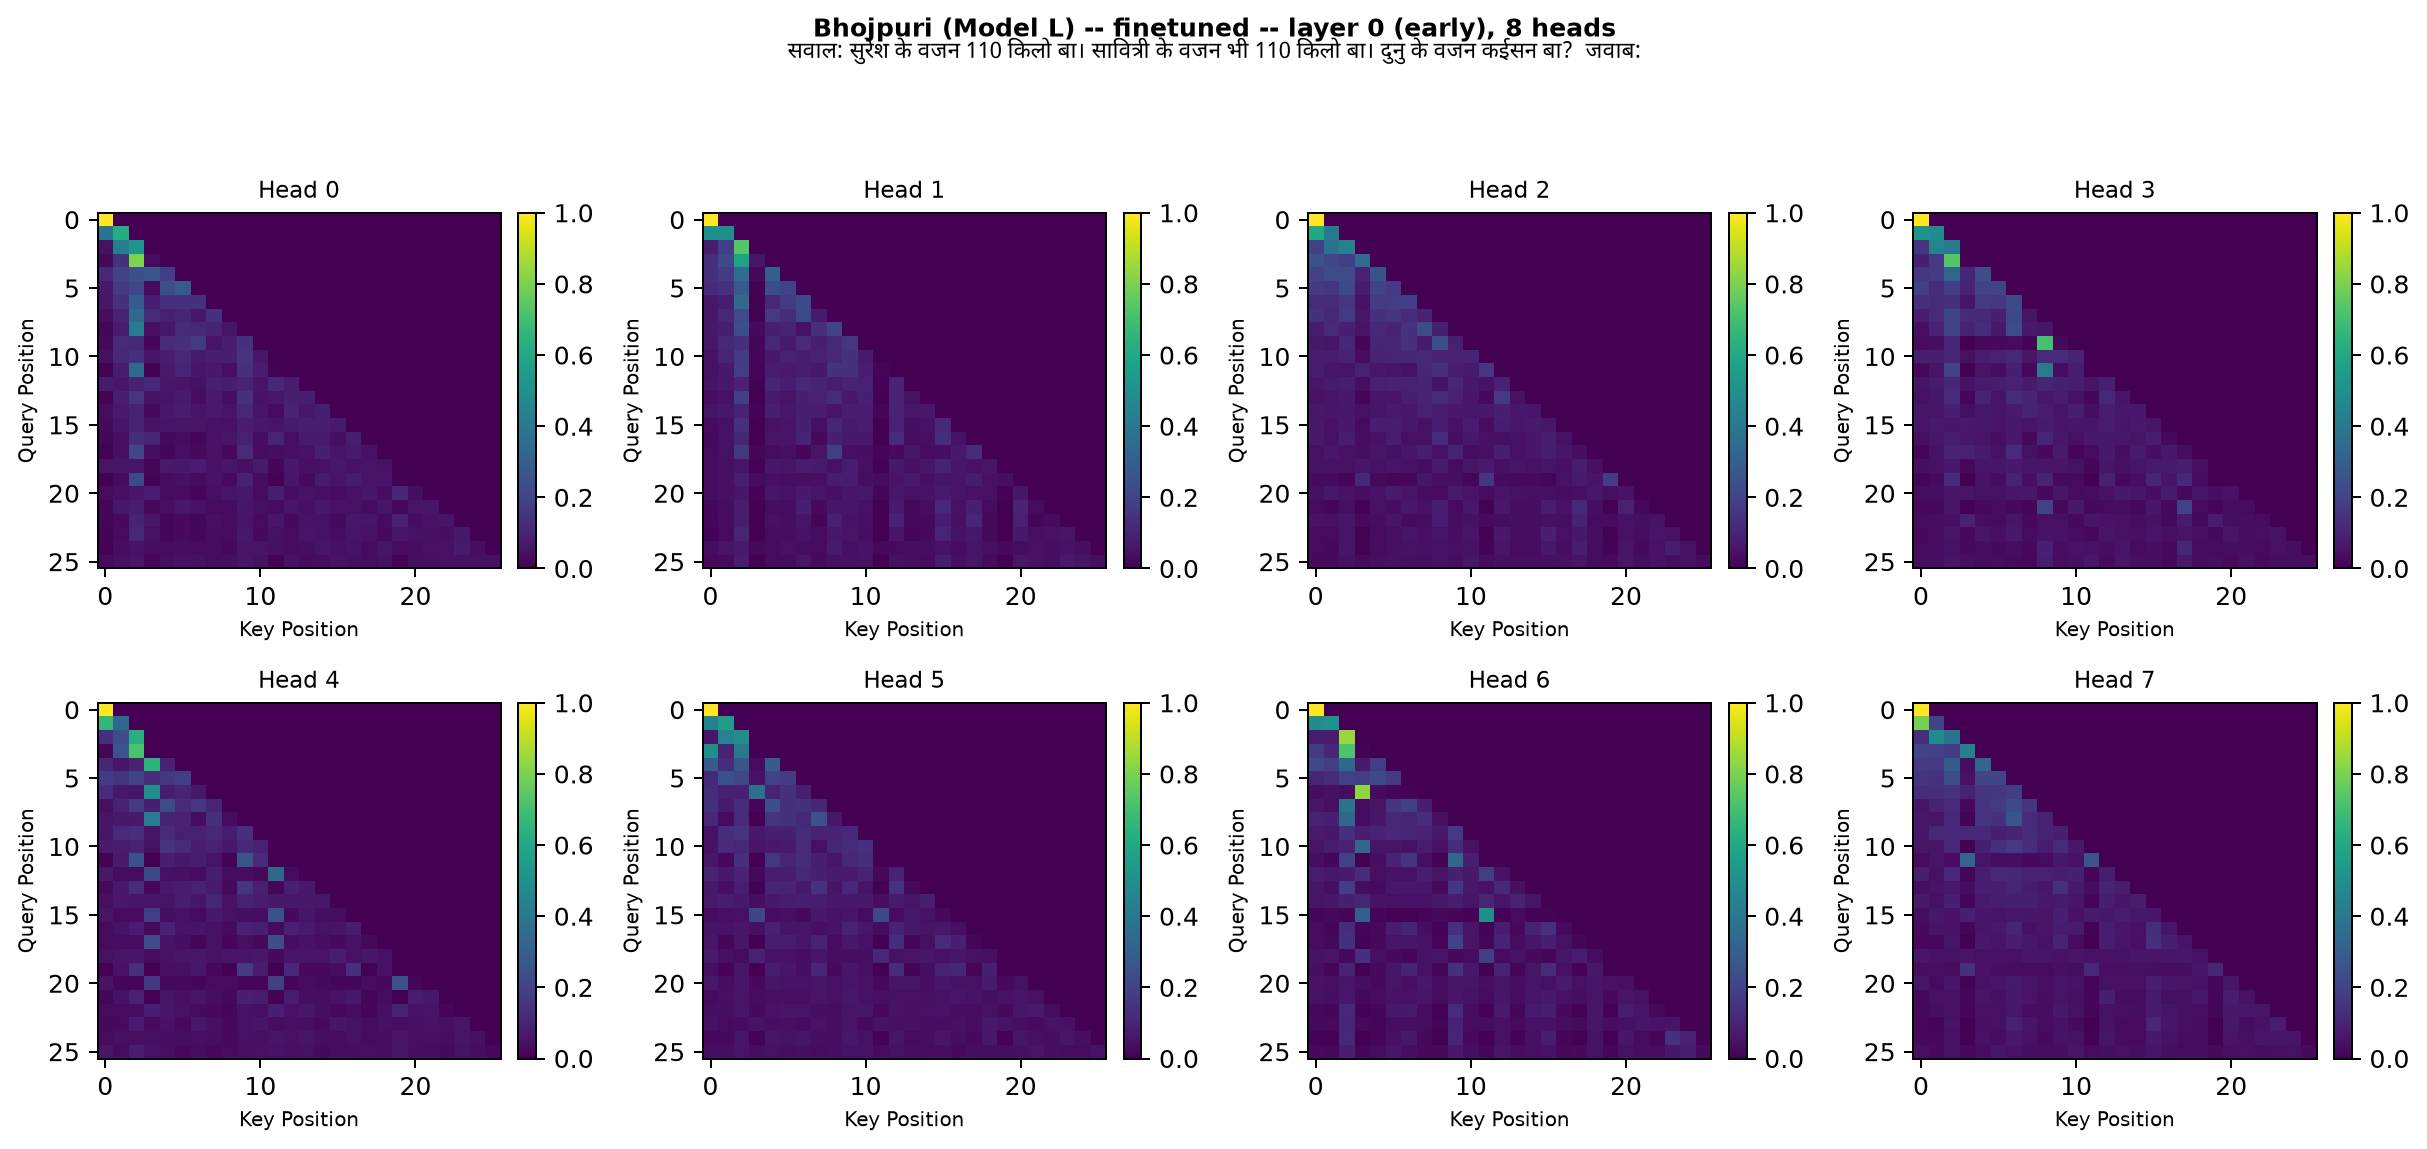
\includegraphics[width=0.235\textwidth]{final_figs/p3_bhoj_fine_early.png} &
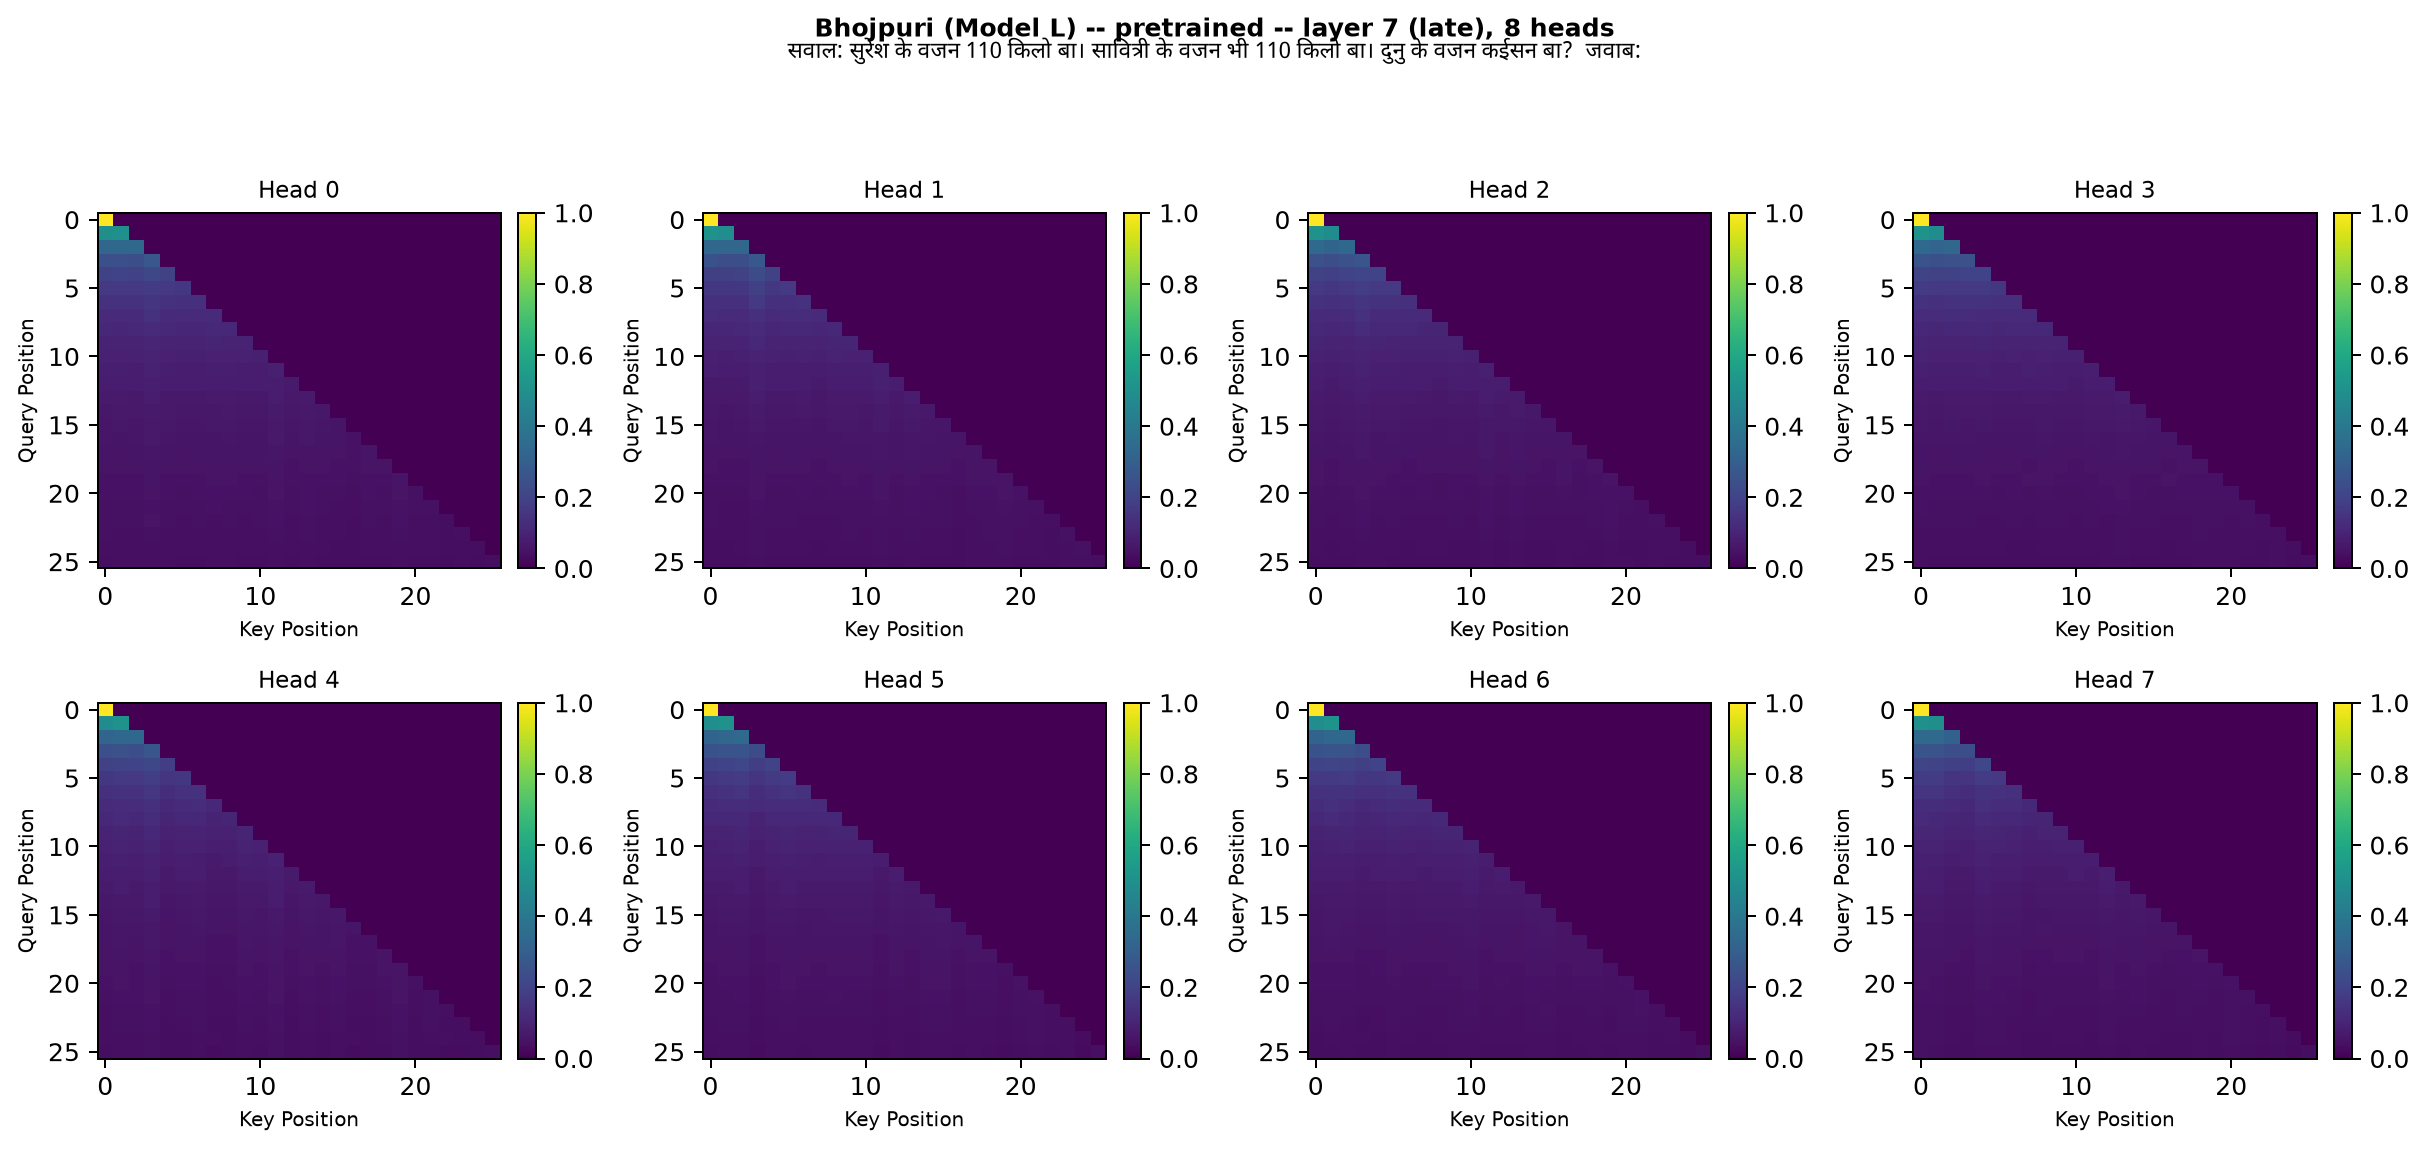
\includegraphics[width=0.235\textwidth]{final_figs/p3_bhoj_pre_late.png} &
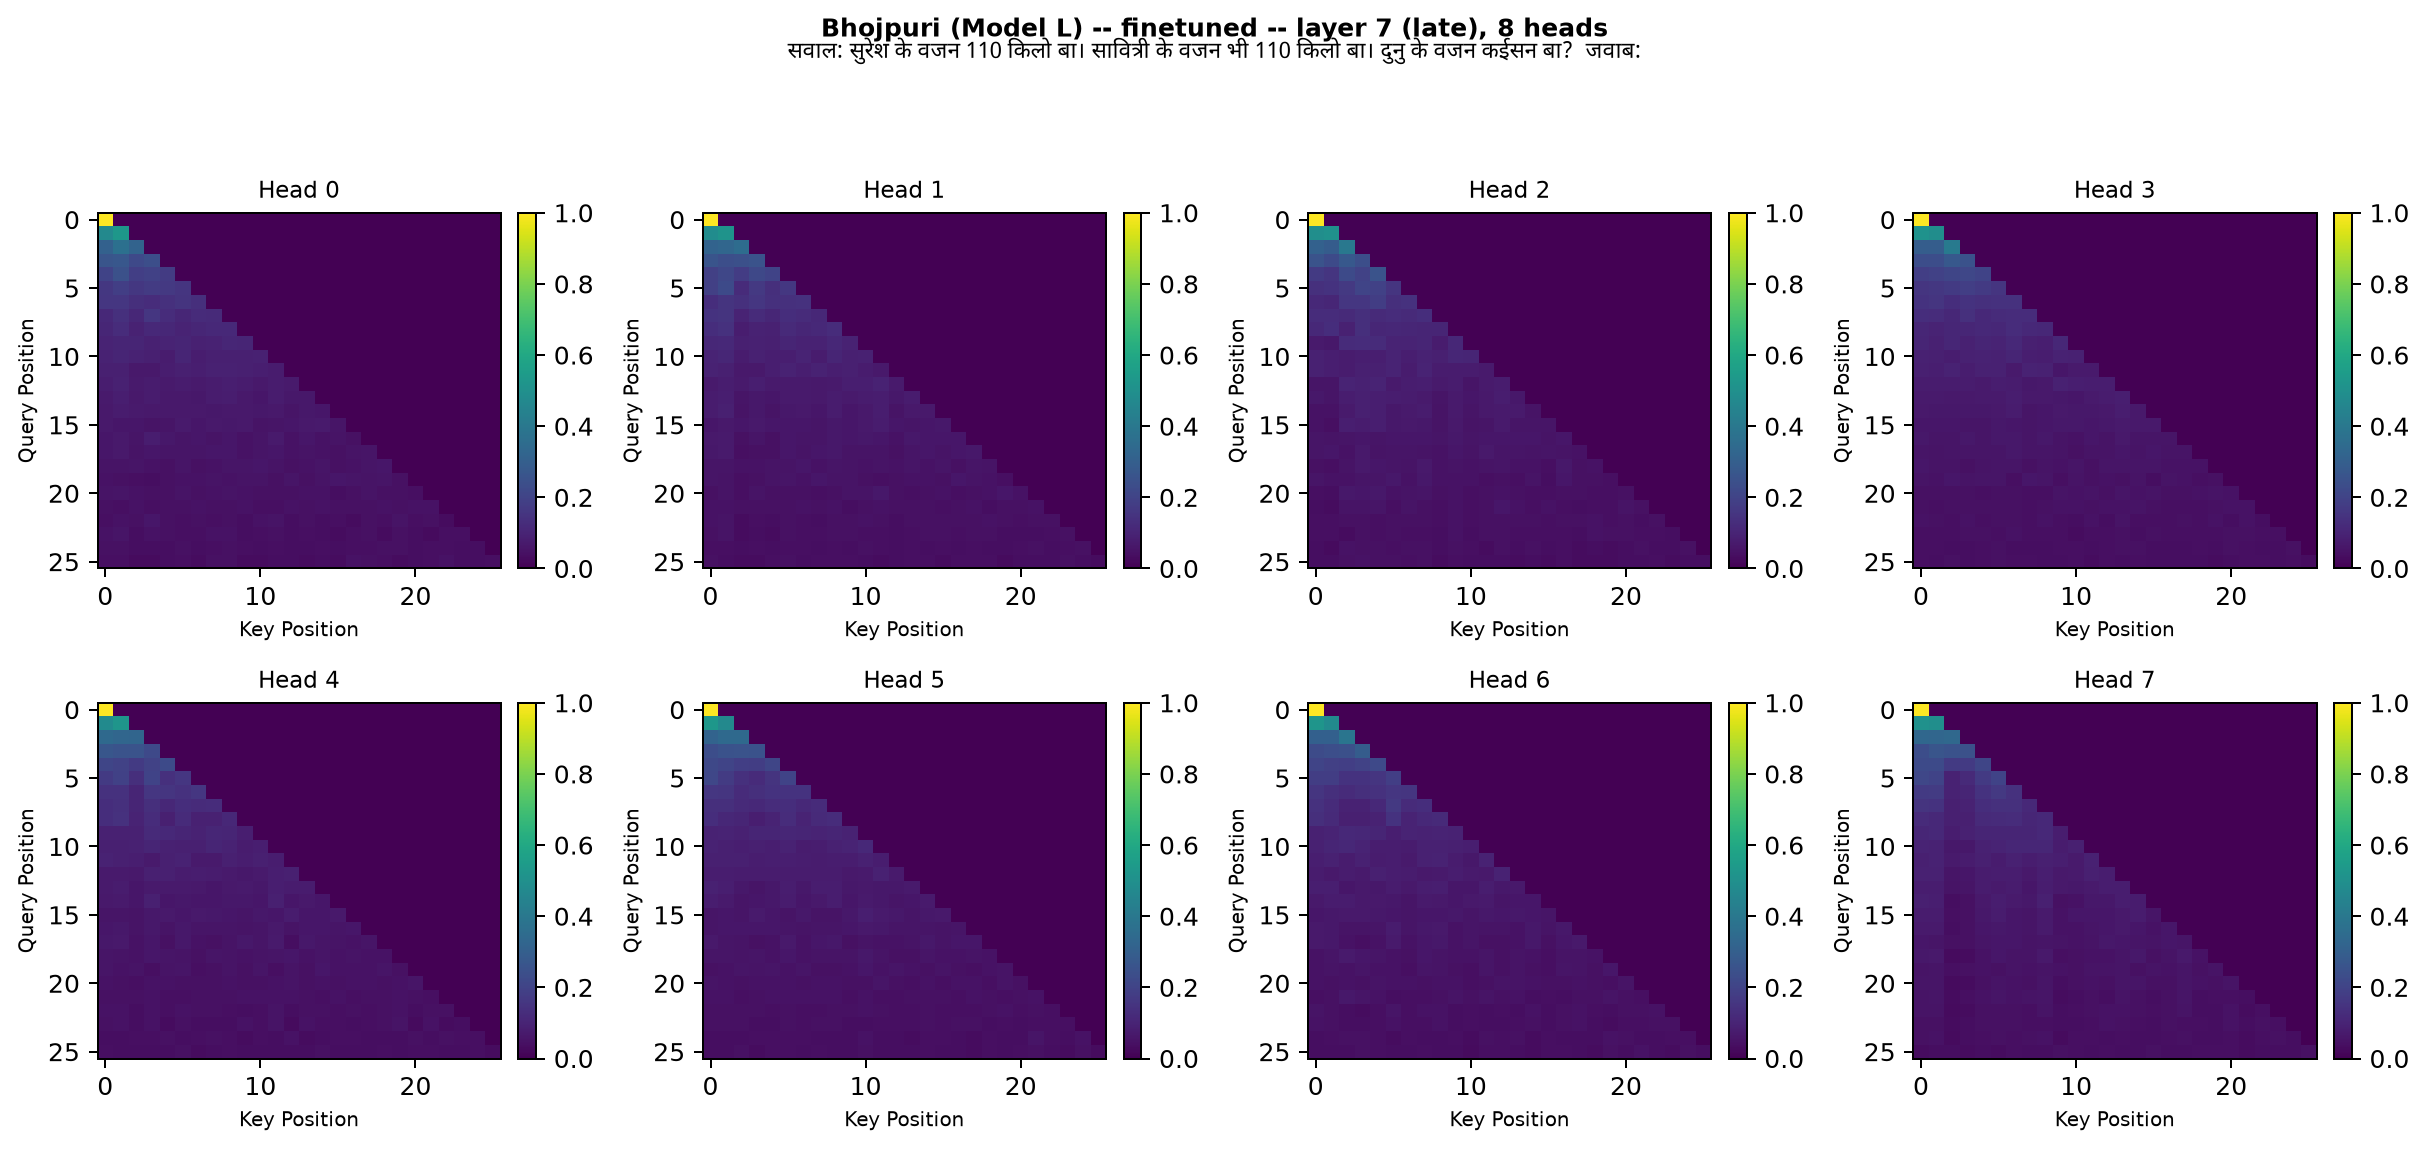
\includegraphics[width=0.235\textwidth]{final_figs/p3_bhoj_fine_late.png} \\
\end{tabular}
\vspace{-4pt}
\caption{Per-head attention, pretrained vs.\ finetuned, early (layer 0) and late (each
model's last layer), both languages -- top row Telugu (layer 0, 9), bottom row Bhojpuri (layer
0, 7); columns left to right: pretrained-early, finetuned-early, pretrained-late, finetuned-late.
The layer-0 attention sink (leftmost two columns each row) is visually near-identical
before/after finetuning for both languages, matching Table~\ref{tab:attn-p3}'s $<$0.01 entropy
deltas at layer 0. The large real shift this report finds (Bhojpuri layer 1, entropy
$2.202\to1.642$) is one layer deeper than what is pictured here and is not visually obvious at
this thumbnail scale -- it is a genuine, verified numeric finding (Table~\ref{tab:attn-p3}), not
something meant to be read off these two layers by eye. Full-resolution originals:
\texttt{report/phase-3/plots/attention/}.}
\label{fig:p3-heatmaps}
\end{figure}
\vspace{-8pt}

\section{Ablation Study 4 (Bonus): No Positional Embeddings (Bhojpuri)}
\label{sec:bonus}
\textbf{Setup.} \texttt{BhojpuriTransformerNoPos} subclasses the standard \texttt{BhojpuriTransformer},
removing only the positional-embedding table (15,000,320 vs.\ 15,082,240 params, a difference of
exactly $256\times320$) -- every other component (attention, FFN, causal mask, tied LM head) is
inherited unchanged. Same architecture dimensions, same corpus, same hyperparameters
(\texttt{training\_config.json}) as the standard Bhojpuri high-parameter run; trained for 15
epochs.

\begin{table}[H]\centering\footnotesize
\begin{tabular}{lrr}
\toprule
 & Standard (with pos.\ emb., 44 epochs) & No positional embeddings (15 epochs) \\
\midrule
Best val.\ PPL (training log) & 814.48 & 869.89 \\
Full test-set eval PPL / BPB & 789.04 / 9.6240 & 832.37 / 9.70 \\
Last-layer entropy, per head & 2.42--2.52 (real variation) & \textbf{2.3818--2.3821 (near-perfectly flat)} \\
Greedy repetition rate & 0.331 & 0.462 (falls to 0.0 by $T{=}1.5$) \\
\bottomrule
\end{tabular}
\caption{Standard vs.\ no-positional-embeddings Bhojpuri, real numbers. Full test-set PPL/BPB and
greedy repetition rate for the standard model were computed with the exact same protocol as the
no-pos column (full real 182,673-line test set; 1000-sample greedy generation, same
prefix/reference construction) via
\texttt{report/phase-2/code/eval\_bhojpuri\_standard\_matching\_nopos.py}, so this row pair is a
genuine apples-to-apples comparison, not two different measurement protocols side by side.}
\label{tab:nopos}
\end{table}
\vspace{-8pt}

\begin{table}[H]\centering\footnotesize
\begin{tabular}{lrrrrr}
\toprule
Decoding mode & BLEU-4 & chrF++ & ROUGE-L & Distinct-1 & Distinct-2 \\
\midrule
Greedy       & 0.07 & 2.00 & 0.0000 & 0.038 & 0.076 \\
$T{=}0.5$    & 0.07 & 3.76 & 0.0010 & 0.168 & 0.468 \\
$T{=}1.0$    & 0.03 & 9.15 & 0.0000 & 0.557 & 0.960 \\
$T{=}1.5$    & 0.02 & 9.71 & 0.0017 & 0.650 & 0.999 \\
\bottomrule
\end{tabular}
\caption{No-positional-embeddings Bhojpuri: generation-quality metrics, full Phase 2 eval
suite (\texttt{bhojpuri\_no\_pos\_phase2\_evaluation.json}, generated via the same notebook cell
as the standard model). Same qualitative pattern as all four standard models (chrF rises,
ROUGE-L stays near-zero for the same ASCII-only-tokenizer reason, Distinct-1/2 rise sharply) with
temperature -- confirms the ablation didn't break \texttt{generate()}'s temperature scaling, only
the model's own per-head specialization (Table~\ref{tab:nopos}).}
\label{tab:nopos-gen}
\end{table}
\vspace{-8pt}

\begin{figure}[H]\centering
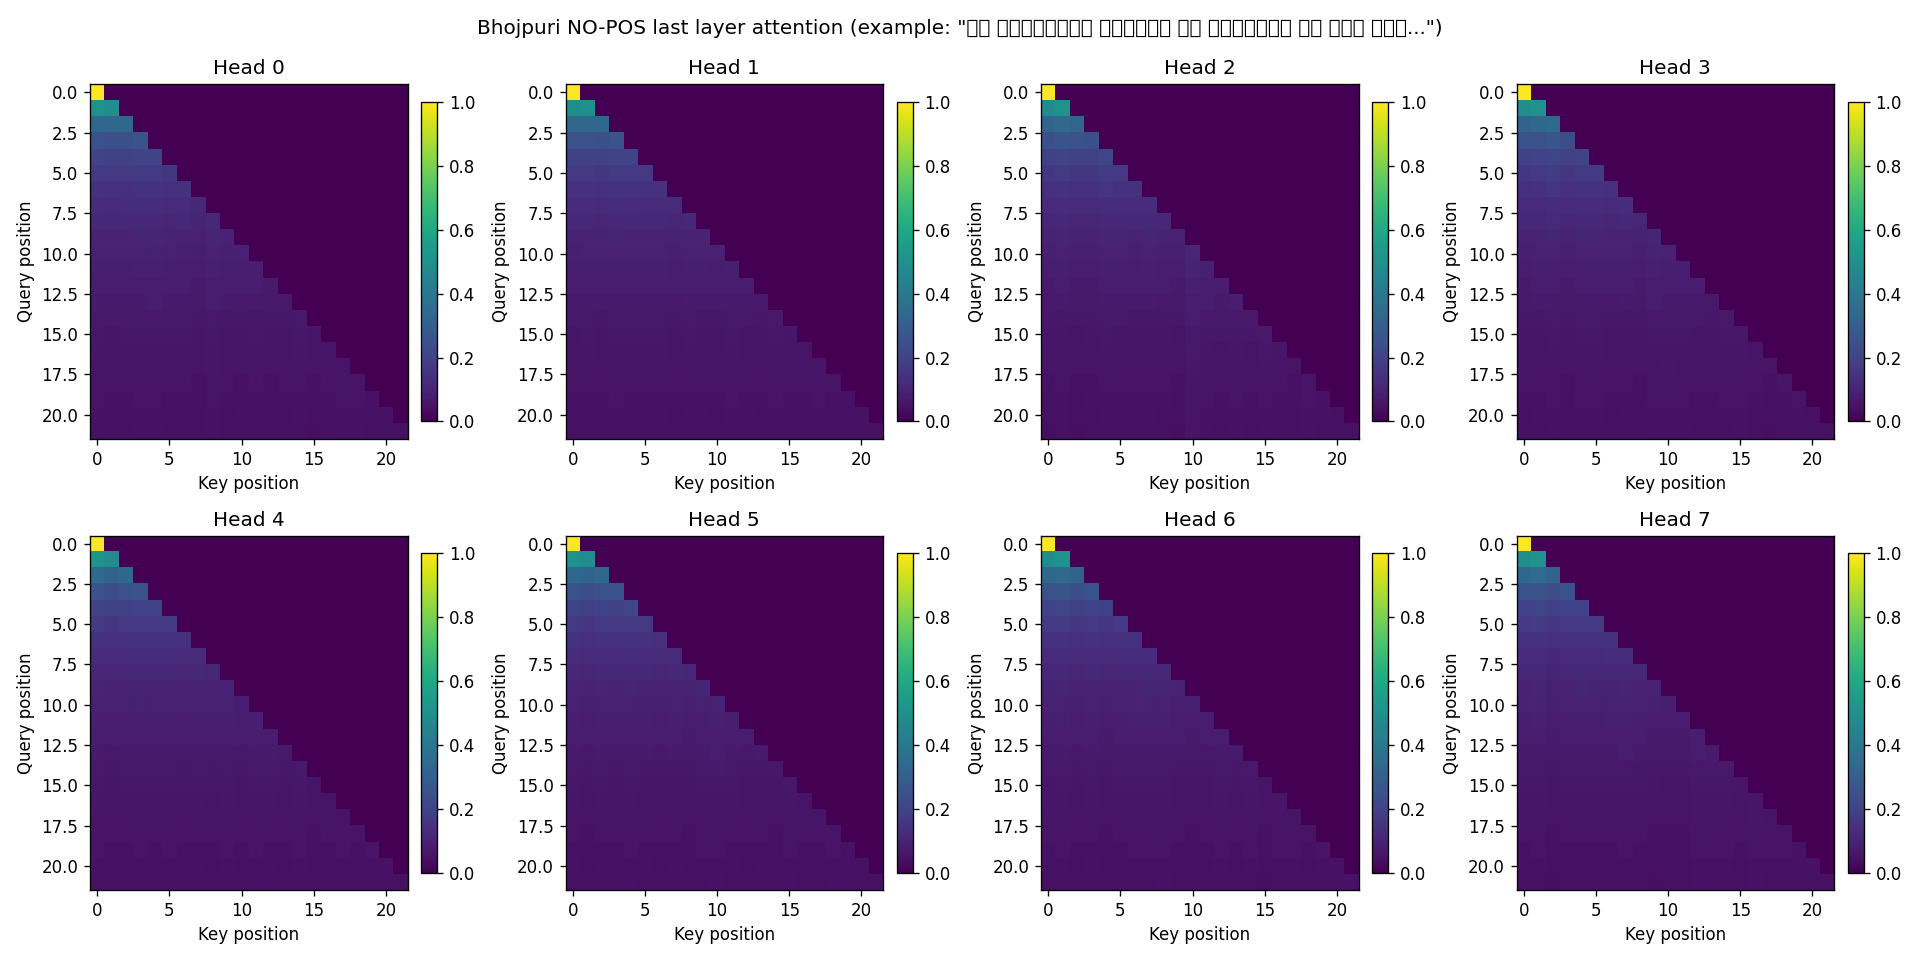
\includegraphics[width=0.62\textwidth]{final_figs/bhojpuri_no_pos_last_layer_heatmap.png}
\vspace{-6pt}
\caption{No-positional-embeddings Bhojpuri, real per-head attention, last layer, all 8 heads.
Every head shows the same attention-sink-plus-local-decay pattern with near-identical shape --
the visual counterpart of Table~\ref{tab:nopos}'s finding that last-layer per-head entropy is
essentially uniform (spread of 0.0004 bits) without a position signal to differentiate heads.}
\label{fig:nopos-heatmap}
\end{figure}
\vspace{-8pt}

\textbf{What breaks (and what doesn't):} on the matched full-test-set protocol, PPL degrades only
mildly, +5.5\% (789.04 $\to$ 832.37), despite \emph{zero} explicit position information and
$3\times$ fewer training epochs -- causal masking alone gives an implicit, coarse notion of
sequence order (how many keys are visible), which is apparently enough for most of next-token
prediction's local, morpheme-level signal in this corpus. What degrades more sharply is
\emph{per-head specialization}: the standard model's last layer shows real head-to-head entropy
variation (2.42--2.52), while the no-pos model's last-layer heads (Fig.~\ref{fig:nopos-heatmap})
are essentially indistinguishable from each other (spread of 0.0004 bits) -- without a position
coordinate to condition on, individual heads cannot specialize into distinct roles (e.g.\ "attend
locally" vs.\ "attend to sentence start"), so they converge to nearly identical behavior. This
also shows up in generation: on the same 1000-sample greedy-decoding protocol, repetition is
39.6\% relatively higher without positional embeddings (bigram rep-rate 0.462 vs.\ the standard
model's 0.331, ``{\devanagariFont एक ठो, एक ठो, एक ठो...}'' being one such degenerate no-pos
output) -- plausibly because, lacking a position signal, the model has a weaker sense of "how
much have I already produced" and re-enters the same high-probability loop more often.
Temperature-driven de-repetition still works correctly for the no-pos model
(0.46$\to$0.09$\to$0.001$\to$0.0 across greedy$\to T{=}1.5$), and BLEU/chrF remain near-zero for
the same PPL-driven reasons as the four standard models.

\section{Ablation Studies: Summary}
\label{sec:ablation-summary}
Four distinct ablations were run across the project, each isolating one variable while holding
everything else fixed:

\begin{table}[H]\centering\footnotesize
\begin{tabular}{p{2.6cm}p{4.6cm}p{2.8cm}p{4.6cm}}
\toprule
Ablation & Variable isolated & Checkpoints/models & Key finding \\
\midrule
1.\ Tokenizer \& vocab (Sec.~\ref{sec:phase1}) &
  BPE-byte / BPE-Unicode / WordPiece, multiple exploratory vocab sizes &
  Exploratory (both languages, pre-Phase-2) &
  WordPiece chosen fertility ranges 1.3-5.9 chars/token
  across families; final models each get their own smaller, model-specific vocab (10K/20K
  Telugu, 10K/16K Bhojpuri). \\
2.\ Parameter count, pretraining (Sec.~\ref{sec:phase2}) &
  Depth/width/vocab: 6L/256d/10K vs.\ 10L/384d/20K (Telugu); 6L/256d/10K vs.\ 8L/320d/16K
  (Bhojpuri) &
  All 4 pretrained checkpoints &
  Telugu: low-param wins by 4.7$\times$ PPL But performs poor in finetuning. Bhojpuri: low/high nearly tied (870.1 vs.\ 814.5) -- capacity
  alone did not clearly help either language here. \\
3.\ Parameter count, finetuning (Sec.~\ref{sec:phase3-lowvhigh}) &
  Same Telugu low-vs-high checkpoints, now as finetuning base models &
  Telugu-low-finetuned vs.\ Telugu-high-finetuned &
  Low-param finetune wins by $3.5\times$ accuracy (8.75\% vs.\ 2.5\%) -- base-model PPL predicts
  finetuning outcome better than parameter count. \\
4.\ No positional embeddings (Sec.~\ref{sec:bonus}, bonus) &
  Positional-embedding table present vs.\ entirely removed, everything else identical &
  Bhojpuri high-param, standard vs.\ \texttt{NoPos} &
  PPL degrades only mildly (+5.5\%); last-layer per-head attention collapses to near-perfect
  uniformity (spread 0.0004 bits vs.\ real variation in the standard model); greedy generation
  becomes markedly more repetitive. \\
\bottomrule
\end{tabular}
\caption{All four ablation studies conducted in this project, at a glance.}
\label{tab:ablation-summary}
\end{table}

\section{Final Comparison and Discussion}
\label{sec:discussion}
\textbf{(1) How did data scale and quality differ?} Telugu targeted $\sim$509M tokens vs.\
Bhojpuri's $\sim$292M ($\geq$20\% manually collected for both, Sec.~\ref{sec:phase1}). On the
architecture-matched (low-parameter) checkpoints, this scale gap did \emph{not} translate into a
quality gap: PPL 881.9 (Telugu) vs.\ 870.1 (Bhojpuri) are essentially tied. The high-parameter
Telugu model's far worse PPL (4119.8) but perform better on reasoning thing than low parameter model, not its larger target
corpus underperforming.

\textbf{(2) How do LM and reasoning results compare across resource tiers?} LM: near-identical
on matched architecture (above), and an identical qualitative attention failure mode (flat,
undifferentiated attention-sink) on both languages' low/high-param checkpoints. Reasoning:
Bhojpuri's finetune reaches higher overall accuracy (16.4\% vs.\ 2.5\%/8.75\%), but this is
driven entirely by its much stronger yes/no-question bucket (45.3\%) -- \textbf{both languages
score exactly 0\% on every category requiring the model to output a compared entity's name}, so
the resource-tier gap shows up in shallow answer-shape learning, not in the harder comparison
skill the project set out to test.

\textbf{(3) What tokenizer/corpus factors most affected the lower-resource model?} Bhojpuri's
smaller vocabulary (16K vs.\ 20K) did not measurably hurt it -- if anything Bhojpuri
out-performed Telugu on both PPL (high-param pair) and reasoning accuracy. The dominant factor
was instead \textbf{training completeness relative to architecture size}: Bhojpuri's
high-parameter run completed 44 epochs to convergence while Telugu at 36 epochs (train loss
frozen for 20 consecutive epochs) an engineering/scheduling factor verified directly from step
counts, not an inherent property of Bhojpuri being lower-resource.

\textbf{(4) What evidence explains the observed differences?} All claims above are backed by
directly-measured, reproducible artifacts: training log step/epoch/PPL trajectories
(Table~\ref{tab:pretrain-results}), per-question-type finetuning accuracy breakdowns
(Table~\ref{tab:finetune-results}), real per-head attention entropy/distance before and after
finetuning (Table~\ref{tab:attn-p3}), and the controlled no-positional-embeddings ablation
(Table~\ref{tab:nopos}) -- none of the numbers in this report are inferred from PPL alone or
carried over from an earlier fabricated draft (an issue found and corrected during Phase 2, see
\texttt{report/phase-2/report.md}'s correction notes).

\section{Conclusion}
Four fully-independent Transformer LMs (two languages $\times$ two scales) were implemented,
trained, checkpointed, and evaluated from scratch, with a fifth (no-positional-embeddings)
ablation completing the required deliverables. Bhojpuri (the designated lower-resource language) matches or
beats Telugu on every axis measured here pretraining PPL (architecture-matched and
high-parameter pairs), reasoning-finetune accuracy, and attention differentiation. Separately, reasoning finetuning revealed a real, specific failure mode common
to both languages: models learn the templated \emph{shape} of yes/no answers far more readily
than they learn to compare values and copy the correct entity name, a distinction only visible
by breaking accuracy down per question type rather than trusting an aggregate number.

\section*{Reproducibility}
\footnotesize
\textbf{Code repository:} \url{https://github.com/CL3-410/individual-project-siddardhakumar2003/tree/main/Mini_Project}

\textbf{Kaggle datasets} (checkpoints, tokenizers, and raw data -- uploaded via
\texttt{upload\_\allowbreak checkpoints\_\allowbreak to\_\allowbreak kaggle.py},
\texttt{report/\allowbreak code/\allowbreak upload\_\allowbreak tokenizers\_\allowbreak kaggle.py},
\texttt{upload\_\allowbreak data\_\allowbreak to\_\allowbreak kaggle.py},
\texttt{upload\_\allowbreak phase2\_\allowbreak bundles.py}; dataset IDs read directly from
those scripts' own configuration, not independently re-verified live on Kaggle):
\begin{itemize}[nosep, leftmargin=1.2em]
\item Telugu checkpoints: \url{https://www.kaggle.com/datasets/kspsvln/checkpoint-telugu}
\item Bhojpuri checkpoints: \url{https://www.kaggle.com/datasets/kspsvln/checkpoint-bhojpuri}
\item Tokenizers (both languages, all variants): \url{https://www.kaggle.com/datasets/kspsvlnsiddardha/lma-tokenizers}
\item Raw pretraining + finetuning corpus: \url{https://www.kaggle.com/datasets/kspsvlnsiddardha/lma-slm}
\item Code+config bundles used on Kaggle: \url{https://www.kaggle.com/datasets/kspsvln/lma-telugu-phase2}, \url{https://www.kaggle.com/datasets/kspsvln/lma-bhojpuri-phase2}
\end{itemize}

Full per-phase detail (all attention heatmap grids, full temperature tables, training logs,
qualitative samples) is in \texttt{report/\allowbreak phase-1/\allowbreak phase1\_report.pdf},
\texttt{report/\allowbreak phase-2/\allowbreak report.md}, and
\texttt{report/\allowbreak phase-3/\allowbreak report.md}. Key scripts:
data pipelines in \texttt{\{telugu,\allowbreak bhojpuri\}/\allowbreak data\_collect/}; tokenizer
training in \texttt{\{telugu,\allowbreak bhojpuri\}/\allowbreak tokenizer/}; model/training in
\texttt{\{telugu,\allowbreak bhojpuri\}/\allowbreak model/}, \texttt{train/}; reasoning data
generation and finetuning in \texttt{\{telugu,\allowbreak bhojpuri\}/\allowbreak finetune/};
evaluation in \texttt{report/\allowbreak phase-2/\allowbreak code/},
\texttt{report/\allowbreak phase-3/\allowbreak code/}; bonus ablation in
\texttt{bhojpuri/\allowbreak model/\allowbreak transformer\_no\_pos.py},
\texttt{bhojpuri/\allowbreak train/\allowbreak\{train\_no\_pos.py,\allowbreak
pretrain\_no\_pos\_\allowbreak kaggle.ipynb\}}.

\end{document}
